%Time-stamp: <2013-06-19 22:33:16 amoebe>
%\documentclass{article}
%\usepackage{graphicx,hyperref} 

\documentclass[12pt]{article}
\usepackage[hmargin=1in,vmargin=1in,letterpaper]{geometry}
\usepackage{lscape}
\usepackage{rotating}
\usepackage{timestamp}
\usepackage{amsmath}
\usepackage{thmtools}
\usepackage{thm-restate}
\usepackage{amssymb}
\newtheorem{hypothesis}{Hypothesis}
\newtheorem{question}{Question}
\usepackage{graphicx}
\graphicspath{ {./figs/} }
\usepackage{caption}
\usepackage{subcaption}
\usepackage{epstopdf}
\usepackage{multirow}
\usepackage{multicol}
\usepackage{tikz}
\usepackage{pgfplots}
\usepackage{tikz-qtree}
\usetikzlibrary{arrows,fit,calc,decorations.markings,positioning}
\tikzstyle{container} = [draw, very thick, dashed, rectangle, rounded
corners, inner sep=2.5em, fill = yellow!20 ]
\definecolor{navy}{rgb}{0,0,0.55}
\definecolor{ruby}{rgb}{0.78,0.15,0.21}
\definecolor{bottle}{rgb}{0.11,0.64,0.22}
\usepackage{standalone}
%\usepackage{subfig}
\usepackage[tone]{tipa}
\let\ipa\textipa
\usepackage{linguex}
\usepackage{hyperref}
\usepackage{natbib}
\usepackage{epsexe}


\title{The experimental state of mind in elicitation: illustrations from
tonal fieldwork \thanks{We thank our wonderful Kirikiri consultant Alfius Polita and
  the other members of the Kirikiri team from the 2011 ANU tone
  workshop: Anthony Woodbury, Rebecca Hetherington, Peter Appleby,
  Rosey Billington, Lea Brown, Isolde Kappus, and Sutriani Narfafan,
  and we gratefully thank Steven Bird, Mark Donohue, Larry Hyman, and
  Mark Liberman for organizing the inspiring tone workshops. We also
  thank Brian Dillon and John Kingston for invaluable
  discussions. This paper is dedicated to Will Leben, my first mentor
  in linguistics.}}
\author{Kristine Yu}
\date{}
\usepackage{graphicx}
\usepackage{fancyhdr}
\usepackage{lastpage}
\usepackage{natbib}
\setlength{\bibsep}{0.0pt}
\setlength{\headheight}{15.2pt}
\setlength{\headsep}{12pt}
\pagestyle{fancyplain}
\fancyhf{}
\lhead{Kristine M. Yu}
\rhead{\timestamp}
\cfoot{\thepage\ of \pageref{LastPage}}

\begin{document}
\maketitle

\abstract{
Inspired by \citet{Hyman:2007,Hyman:2001}, we cast fieldwork
elicitation with an experimental state of mind. We begin by
illustrating how principles of experimental design underlie
\citet{Pike:1948}'s classic toneme discovery procedure. These
principles include the consideration of confounding variables that can
obscure the relation between the manipulated independent variable and
the affected dependent variable, as well as the explicit statement of linking hypotheses about
the map between unobservables, like tonal concepts, and quantities we
can use to indirectly observe them, such as pitch patterns. We show
that recognizing the role of these principles in toneme discovery
allows us to use the same principles to generalize to elicitation
methodology for fieldwork ranging from acoustic studies of tonal
realization to explorations of tonal allophony and alternation and the
syntax-prosody interface.  We close with an in-depth look at
considerations for linking hypotheses between tonemes and observable
phonetic parameters of the voice source.
  
}

\section{Introduction}
\label{sec:intro}

This paper revisits a very old method for studying tone languages:
``how do you say X?'' Summed up like this, elicitation from
linguistic consultants might not seem to have the capacity to be particularly well-defined or
rigorous as a method. But that would be a mischaracterization, as is
evident from \citet{Pike:1948}'s brief summary of elicitation
methodology for discovering tonemes in his classic tome on how to study a tone language:

\begin{quote}
\textsf{The procedure indicated is basically a method of controlling free,
conditioned, key, mechanical, morphological, and sandhi tonal changes
by inserting lists of words into selected contexts so as to reduce the
number of variables at any one time and give the investigator the
opportunity of observing the significant linguistic pitch in its
simplest contrastive forms \citet[p.\ vii]{Pike:1948}'s.  }
\end{quote}

Pike's description evokes an \textit{experimental state of mind} in
elicitation.  By referring to the experimental state of mind, we take inspiration
 from \citet{Hyman:2001}'s conception of fieldwork as a state of
 mind: just as Hyman remarks that ``it is possible to be a
fieldworker without constantly going to the field,'' so is it
possible to be an experimentalist in pursuing fieldwork without ever
stepping foot in a lab. Bringing the lab to the field, e.g.\
conducting psycholinguistic experiments in the field, is a burgeoning
line of research---see for instance, the forthcoming special issue of
\textit{Language and Cognitive Processes}, Laboratory in the Field \citet{Jaeger:2014}. However, the
focus of this paper is how an experimental state of mind can
inform and enrich traditional elicitation methodology in fieldwork.

 In this paper, we expound upon \citet{Hyman:2007}'s
remark that ``elicitation is experimental phonology'' and illustrate
how to guide elicitation in terms of experimental design and
analysis. The principles illustrated are applicable regardless of the
linguistic phenomenon and data being elicited, but for this paper, we
focus on: (1) the problem of discovering the tonemes of a language and
(2) how to elicit and analyze phonetic data to tackle this problem. We
present illustrative examples from our experiences in
discovering the tones of Kirikiri (Papua New Guinea, Lakes Plain) in
fieldwork conducted with team members at the Prosodic Systems in New
Guinea Workshop in December 2011, supplemented by experiences in
fieldwork on Samoan (Samoa, Polynesian), Mandarin (China,
Sino-Tibetan), and Cantonese (China, Sino-Tibetan).

 The structure of the rest of the paper is as follows: we begin by
 using Pike's toneme discovery procedure as a starting point for
 illustrating the role of experimental design in elicitation in
 \S\ref{sec:components}. Then, we show how we can use principles of
 experimental design to generalize beyond Pike's elicitation methods
 in tonal fieldwork in \S\ref{sec:generalize-exp-design}. Since
 assumptions about how we can observe reflexes of directly
 unobservable tonemes underpin any conclusions we can draw
 in elicitations, we close in \S\ref{sec:pitch}
 with an extended discussion of a key component of the experimental design---the map between the unobservable
 cognitive concept of a toneme and observable acoustic and perceptual
 properties of speech, including f0 and pitch and beyond. 

In addition to the body of the paper presented here, a major component
of the paper is a set of tutorials on collecting and analyzing
phonetic data from elicitations. These tutorials and supporting files
are referred to in the body of the paper and presented as supplementary
material online at \url{www.krisyu.org} and
\url{www.github.com/krismyu/ldc-kiy}. We've chosen to prepare on-line
tutorials to facilitate interactivity with code and supporting media.


\section{Components of an experimental state of mind}
\label{sec:components}

In this section, we walk through \citet{Pike:1948}'s toneme discovery
algorithm (\S\ref{sec:pike-toneme}) and then show how it can be
conceived as an application of principles of experimental design in
two stages (\S\ref{sec:pike-toneme-early}, \S\ref{sec:pike-toneme-design}). 

\subsection{\citet{Pike:1948}'s toneme discovery procedure: a walkthrough}
\label{sec:pike-toneme}

Pike's elicitation methodology for discovering tonemes in
\citet[Ch.\ IV, p.\ 48-54]{Pike:1948} consists of two
main steps:\footnote{Pike further describes methods for
  determining the number of tonemes and their phonological description
  in Ch.\ V, but we focus on his first two steps for the purposes of
  illustrating the experimental state of mind in elicitation in this paper.}
\begin{enumerate}
\item Classification of words into
  word classes (\textit{substitution lists}) of uniform morpho-phonological structure 
\item Classification of words into groups that are tonally uniform in
  controlled contexts
\end{enumerate}

Figure \ref{fig:pike-tikz} schematizes the entire two-step procedure;
Figure \ref{fig:words-tikz} illustrates the first step of
classification of words into word classes in detail, and Figure
\ref{fig:sub-tikz} exemplifies the second step of examining the tonal
properties of words in controlled contexts.

\begin{figure}
  \centering
  \includestandalone[width=\textwidth]{pike-tikz}%     without .tex extension
  \caption{A schematic summarizing the discovery procedure for tonemes
    in \citet[Ch.\ 4]{Pike:1948}. There are two main steps: (1)
  classification of words by morpho-phonological structure into word
  classes (\textit{substitution lists}), and for each substitution list, (2)
  classification of the items in the list into tentative tonal classes by their
  pitch patterns in a phrasal (possibly sentential) context, a \textit{substitution frame}. The second step is
  repeated for all applicable substitution frames for the substitution
list, for all substitution lists, and proposed tonal classes may be
adjusted after each iteration. Abbreviations: TBU = tone bearing
unit, N = noun, V = verb, Adj = adjective.}
  \label{fig:pike-tikz}
\end{figure}

As Pike states, the purpose of the first classification of words by
morpho-phonological properties is to control properties of the words
such that any variation in pitch patterns of words is highly likely to
be due \textit{only} to tonemic contrast: 

\begin{quote}
  \textsf{\small{The first classification brings together words which
      are somewhat alike in phonetic and grammatical structure. Such a
    grouping tends to reduce the hazards introduced in the analysis of
  these words by segments which cause nonphonemic modification of
  tonemes. The ear is distracted in its listening for pitch when the
  forms of the items under attention are not comparable. \citep[p.\ 48]{Pike:1948}}}
\end{quote}


\begin{figure}
  \centering
  \includestandalone[width=\textwidth]{words-tikz}%     without .tex extension
  \caption{A classification tree depicting the initial step of partitioning
    words by morpho-phonological structure in the discovery procedure for tonemes
    in \citet[Ch.\ 4]{Pike:1948}. Words are partitioned by lexical
    class, length (in syllables), CV skeleton, and segmental
    features (here, onset voicing). The sets of terminal elements
    $\{ba, da,$\ldots$\}$, $\{pa, ta,$\ldots$\}$ are word classes Pike calls
    \textit{substitution lists}. These word classes are uniform in morpho-phonological
    structure and are to be elicited in controlled contexts in the second step
    of the discovery procedure.}
  \label{fig:words-tikz}
\end{figure}

The morpho-phonological properties listed for consideration in this
first classification step in Figure \ref{fig:words-tikz} (lexical class, length,
CV-skeleton, etc.) should not be taken to be a rigid prescription for
exactly how to partition words into classes for pitch pattern
comparison. The set of properties listed may
be neither necessary nor sufficient for toneme discovery in a
particular language. Moreover, the output word classes, the
\textit{substitution lists} from the
classification, may well be adjusted in the course of fieldwork to yield
a coarser or finer-grained partition of the words. For instance, the
classification tree in Figure \ref{fig:words-tikz} currently does not
distinguish vowel quality, but in the course of tonal fieldwork, if one
suspected an interaction between vowel height and pitch patterns,
a natural step would be to include vowel height in word
classification. This heightened attention to vowel quality in classification would yield a
finer-grained partition of the words and introduce an additional level
of depth to the classification tree.    

The output of the first classification step, the word classes Pike
calls \textit{substitution lists}, is the input to the second classification
step schematized in Figure \ref{fig:sub-tikz}. For each substitution list, a set of
\textit{substitution frames} is generated. As shown in the middle box labeled
``substitution frames'' in Figure \ref{fig:sub-tikz}, the
specification of these frames includes phrasal-level prosodic
structure as well as pragmatic context.\footnote{\citet[p.\
  51]{Pike:1948} actually discusses controlling ``emotional
  context$\ldots$ to prevent intonational changes''. We take
  ``emotional context'' to have a meaning
  roughly equivalent to that of that of
  \textit{pragmatic context} as a cover term for situational context
  that may interact with prosody.} For each iteration of eliciting a
substitution list in the context of a substitution frame, the items in the
substitution list are sorted into tentative tonal groups by their particular
pitch patterns in the substitution frame. Comparison of hypotheses for tonal
groupings from different substitution frames for a substitution list
provides converging or diverging evidence for particular proposed
tonemes. These hypotheses may eventually also be compared to
generalize not only over substitution frames within a substitution
list, but also across substitution lists. 

A final important point about
the tonal classification step is the emphasis on the assignment of
group labels to words rather than the nature of the labels
themselves. Pike writes that: ``up to this
point there has been no essential need for tonal transcription. It is
the grouping as such which has been important'' \citep[p.\
55]{Pike:1948}: in Figure \ref{fig:sub-tikz}, what's critical in the
rightmost ``pitch
patterns'' box is not the IPA tonal transcription, but the colors of the
boxed tones, which indicate group membership.\footnote{This
  observation about the importance of sorting and clustering pitch
  patterns in contrast to the negligible role of the choice of
  representation of pitch patterns in the early stages of toneme
  discovery, also discussed at the Berkeley Tone Workshop in 2011 (NSF
  Project Prosodic Systems in New Guinea: Integrating computational and typological approaches to linguistic analysis), was the key motivation for the development of
  computational software to aid this clustering (see this
  volume).} 

The output of Pike's second toneme discovery step can be thought of as
a list of mappings from words to glass jars in a pantry storing jars of words. We
might have faded written labels on the jar lids, but what really
serves as the jar labels in the pantry is the set of identifying and
distinguishing properties of the contents inside a jar. Indulging a
bit with this pantry metaphor: take a shelf storing various kinds of
pasta---we might not know whether to label a jar as \textit{gemelli} or
\textit{bucatini}, but it's easy enough to keep the different pasta
jars straight and to glance at the jars and get down ``the jar with the little
spirals'' as opposed to ``the jar with those long tubes.'' We discuss
considerations for the nature of tonal class labels further in
\S\ref{sec:pitch} when we examine the map between tonal classes and
acoustic and perceptual dimensions. 


\begin{figure}
  \centering
  \includestandalone[width=\textwidth]{sub-tikz}%     without .tex extension
  \caption{A schematic summarizing the second step in the discovery
    procedure for tonemes in \citet[Ch.\ 4]{Pike:1948}. This consists
    of eliciting items
    in a word class (substitution list) $\mathcal{W}_{\gamma}$ in a
    substitution frame $\mathcal{F}_j$ (boxed in yellow) among the
    substitution frames licit for $\mathcal{W}_{\gamma}$ and sorting the items by pitch
    pattern into tentative tone classes (tonemes). Frame
    $\mathcal{F}_j$ positions items utterance-medially in a particular
    pragmatic context $prag2$. The elicited pitch patterns (transcribed with
    IPA tone symbols) for
    $\mathcal{W}_{\gamma}$ in $\mathcal{W}_{\gamma}$ are clustered
    into tentative tone classes. For simplicity, we assume that the
    substitution items are monosyllabic and that there is one tone per
    syllable. Here, $w_{\gamma
      2}$ and $w_{\gamma i}$ are proposed as members of a tentative
    tone class (colored bright green)
    since they share a pitch pattern in context $\mathcal{F}_j$
    distinct from the pitch patterns in $\mathcal{F}_j$ for other words in $\mathcal{W}_{\gamma}$.}
  \label{fig:sub-tikz}
\end{figure}

Now that we've laid out Pike's toneme discovery procedure, we
unpack it into two sequential stages: (1) treating tonal class as a
\textit{latent variable}, as something to infer from the unexplained
variability in pitch contours over words (\S\ref{sec:pike-toneme-early}), and (2) explicitly manipulating
(putative) tonal classes as \textit{independent variables} in testing
hypotheses about the partition of words into tonal classes
(\S\ref{sec:pike-toneme-design}). We provide running illustrations of
each stage from fieldwork on Kirikiri.

\subsection{Experimental design in early toneme discovery: tonal class
  as a latent variable}
\label{sec:pike-toneme-early}

At the earliest stages of studying a language, we may not be even sure
if it has lexical tonal classes, and even if we are confident that there does exist
tonal classes in the language, we don't know enough about them to manipulate \textsc{tonal
class} as an \textit{independent variable} and explicitly group
words into different tonal classes.\footnote{Note that the independent variables are manipulations of each
elicitation item constructed and elicited by the fieldworker (the
\textit{experimental unit}) and uttered by the consultant, not
manipulations of words in the language of study. When we discuss
manipulating syllable structure or tonal class as independent
variables, we are not claiming
to manipulate the syllable structure or tonal class of a word (that's left to nature! Such a
study with the word rather than the elicitation item as the
experimental unit would not be an experiment, but an
\textit{observational study} \citep{Rosenbaum:1999}.) Instead, we
manipulate the properties of an elicitation item---properties of the
substitution frame, as well as properties of the target word,
including the tonal class of the target word within the elicitation
item. Throughout this paper, when we refer to any independent or
dependent variable, we always mean to refer to the variable associated
with the experimental unit of the elicitation item, e.g.\ 
``the pitch contour over a word'' is short for ``the pitch contour
over a word embedded in an elicitation item uttered by the consultant
in an elicitation session.''}
 Our research hypothesis at this
point is:

\begin{hypothesis}[Existence of tonal classes]
\label{hyp:tones} There are tonal classes in Kirikiri.
\end{hypothesis}

Note that tonal classes are not directly observable: we can only indirectly observe the
presence of tonal classes through the \textit{dependent variable} of
the pitch contour over the word, which we observe as we elicit each
new item with our consultant. As is implicit in Pike's procedure,
in order to proceed in discovering hidden structure which is not
directly observable, we must make assumptions linking properties of
speech that we can observe---\textit{observed variables}---to unobservable, underlying
tonal classes---\textit{latent variables}. Such assumptions can be encoded in a \textit{linking
hypothesis}, which makes explicit assumptions about the relation
between observed variables, e.g.\ pitch contours over words, and
(unobserved) latent variables, e.g.\ tone classes:\footnote{Some of
  the earliest discussion of linking hypotheses in studying human
  behavior comes from the study of human vision \citep{Brindley:1960},
  in which linking hypotheses must be made about the mapping between
  perceptual and psychological states. Here, we're also making
  linking hypotheses about the mapping between perceptual (auditory) states
  (pitch contours over words) and psychological (cognitive) states
  (tonal concepts---tonemes).  See \citet{Teller:1984} for a
  historical perspective and some philosophical discussion and
  \citet{Yurovsky:2012} for current work on linking hypotheses.}
\begin{restatable}[Linking hypothesis between lexical tone classes and
  pitch contours]{hypothesis}{link}
\label{hyp:link1}
Lexical tone classes (tonemes) induce systematic variation in the
pitch contours of words. Therefore, the unobservable cognitive concept
of a toneme is observable via its influence on the pitch contours of
words: if two words have different pitch contours, then they belong to
different lexical tonal classes.
\end{restatable}

This linking hypothesis in Hypothesis \ref{hyp:link1} should make the
reader sputter with incredulity: what about all the other potential sources of influence on the
pitch contours of words uttered during an elicitation that we've been
discussing in \S\ref{sec:pike-toneme}? Suppose, for instance, that we
elicited one word at the end of the utterance and another one in the
middle of the utterance. If these two words were uttered with different
pitch contours, and we concluded on the basis of Hypothesis
\ref{hyp:link1} that the two words belonged to different tonal
classes, we could be mistaken: perhaps the pitch differences were
actually due to the difference in prosodic position between the two
elicited utterances. 

There is still a sense in which Hypothesis \ref{hyp:link1} is
reasonable, though. \textsc{Lexical tone class} could certainly be \textit{one}
variable in a model explaining variability in the pitch contour over a
word, and \textsc{prosodic position} and any other of the
variables mentioned in \S\ref{sec:pike-toneme} could be \textit{explanatory
variables} as well---independent variables that are
central to our research questions and hypotheses. There could be \textit{many} explanatory variables in a
model of pitch contour variation. In order to provide
evidence that \textsc{tonal class} is one of these explanatory
variables (Hypotheses \ref{hyp:tones} and \ref{hyp:link1}), we follow
the strategy below:  

\begin{itemize}
\item Propose a set of independent variables to include in a model to explain pitch
contour variation. This set does not include \textsc{tonal class},
since we are not yet at the stage where we can manipulate
\textsc{tonal class} as an independent variable. 
 
\item See how far the set of explanatory variables in our model
goes towards explaining the variability in pitch contours of words
from elicited utterances.
\begin{itemize}
  \item If the leftover unexplained
variability is huge,\footnote{In statistical data analysis, what
  counts as ``huge'' is precisely defined in terms of the ratio of
  unexplained variability to total variability, but for application in fieldwork
elicitation, an intuitive definition of ``huge'' is sufficient.} we suspect that we may have missed one or more important
explanatory variables in our model, and if we have considered a
sufficiently wide range of possible variables for our model, then we can
conclude with some confidence that we need to have \textsc{tonal class} in the model
to help explain the pitch contour variability. (Figure
\ref{fig:unexplained}) We can then proceed to check if we have a big
gain in explained variance with \textsc{tonal class} in the model. 
\item If the leftover unexplained variability is small, we have no
compelling positive
evidence for the language having lexical tonal classes. The small
proportion of variability left unexplained is likely due to a
constellation of secondary influences on pitch contour variation we've
abstracted away from, e.g.\ various sources of elicitation
session-to-elicitation session variability, as discussed further in \S\ref{sec:gen-iv}. (Figure \ref{fig:explained})
\end{itemize}
\end{itemize}

Under this strategy, we begin with a morass of variability in the
pitch contour over a word (Figure \ref{fig:noise}). None of this
  variability is explained, i.e.\ all of the variability is
  \textit{unexplained}. Upon introducing variables into a model of
  pitch contour variation, we hope to be able to carve off some of
  that variability into \textit{explained variability}, variability
  which is accounted for by our introduced explanatory variables. The
  better we understand what influences pitch contour variability, the
  more variability from the total variability that we are able to partition
  into \textit{explained variability} and the less that remains
  \textit{unexplained variability}. If our model does not do a good job of
  covering the sources of influence for pitch contour variability, the
  partition between explained and unexplained variability looks
  like the breakdown in Figure \ref{fig:unexplained}, where most of the
  variability remains unexplained. If our model does
  in fact do a good job, then the partition looks like the decomposition
  in Figure \ref{fig:explained}, where most of the variability is
  explained by the proposed explanatory variables.  

\begin{figure}
  \centering
\subcaptionbox{No variability explained\label{fig:noise}}
[.4\linewidth]{\includestandalone[width=0.04\textwidth]{triangle3-tikz}}%
\qquad\qquad
\subcaptionbox{Most of the variability unexplained\label{fig:unexplained}}
[.4\linewidth]{\includestandalone{triangle-tikz}}%

\hfill\break

\begin{subfigure}[t]{0.5\textwidth}
  \centering
  \includestandalone[width=\textwidth]{triangle2-tikz}%     without
  \caption{Most of the variability explained}
  \label{fig:explained}
\end{subfigure}
  \caption{A geometric 
summary of partitioning the total variability in the pitch
  contour over a word into two parts \citep{Saville:1986}: (1) the variability explained,
  i.e., the variability accounted for by the independent variables given
  in Table \ref{tab:pike-iv}  and
  (2) the residual (unexplained) variability, which must be attributed to the influence
  of variables not enumerated in Table \ref{tab:pike-iv}---in
  particular, we hypothesize, the influence of the latent variable \textsc{tonal class}.}
  \label{fig:triangle-tikz}
\end{figure}

At this point, our guiding research question is:

\begin{question}[Explaining variability in pitch contours]
Can we explain part of the variability in the pitch contour over a word in an
elicited utterance? How much of this variability can we explain?
\end{question}

What explanatory variables should we include in a model of pitch
contour variability? The answer from Pike's procedure is Hypothesis
\ref{hypothesis:variance}---the variables to include are in the list of
variables we discussed in \S\ref{sec:pike-toneme}, which we summarize
in Table \ref{tab:pike-iv}. Unlike \textsc{tonal class}, we know
enough about the variables in Table \ref{tab:pike-iv} to manipulate
them as independent variables. For instance, we can explicitly
manipulate the \textsc{syllabic length} of the target word in an
elicitation item to be set at different \textit{levels}---possible
instantiations of a variable in the experimental design, e.g.\
monosyllabic, disyllabic, etc.

\begin{hypothesis}[Explaining variation in pitch contours over words]
\label{hypothesis:variance}
The primary influences on variation in pitch contours over words are
the variables listed in Table \ref{tab:pike-iv}.
\end{hypothesis}

\begin{table}[!h]
  \centering
  \begin{tabular}{l | l}
    Variable & Examples of levels\\\hline
    Lexical class &  noun, verb\\
    Morphological complexity &  simplex, complex\\
    Syllabic length &  monosyllabic, disyllabic\\
    CV skeleton &  CV, CVC, CCV, CV:\\
    (Vowel length) &  (short, long)\\
    Segmental features &  intial voiced stops, initial
    voiceless stops\\
    Stress &  Present, absent\\
    Stress assignment &  Initial, peninitial, 3rd
    syllable, penultimate\\\hline
    Prosodic position &  utterance-initial, isolation\\
    Pragmatic context &  Out of blue focus, contrastive
    focus on first NP\\
    Syntactic structure &  Possessive prenominal phrase, relative clause\\
  \end{tabular}
  \caption{Independent variables in \citet{Pike:1948}'s toneme
    discovery procedure. The table gives each variable name,
    and a couple examples of levels---possible instantiations of a variable in the
    experimental design, e.g.\ \textsc{lexical class} = noun;
    \textsc{lexical class} = verb. A horizontal line divides variables
    pertaining to the word (items in the substitution lists) and
    variables pertaining to the context (substitution frame). Vowel
    length is listed in parentheses since Pike mentions it explicitly,
    but it could also be subsumed under CV skeleton. }
  \label{tab:pike-iv}
\end{table}

  We should not delude ourselves that the small list of variables in
Table \ref{tab:pike-iv} exhaustively captures all aspects of the
elicitation context in toneme discovery that may influence pitch
contour variation over a word, since context is always
unbounded (Is the consultant lethargic or excited? How far away are
you sitting from the consultant? What were the last five words
elicited---has the consultant started building a discourse context
around them? What time of day is it?  How much sleep did the consultant
get last night?). However,
we can try to capture the primary aspects of relevant context: we can
tackle contextual variables that we know of and that we suspect may
account for a large amount of variability in the pitch contour of a
word in an elicited utterance. There'll always be variability left
unexplained.\footnote{It is typical in psycholinguistic studies for
  most of the variability in the dependent variable (which is
  frequently reaction time in a subject's response to some stimulus)
  to be due to variability among subjects and items: the explanatory
  power from the variables of interest is swamped by
  subject-to-subject and item-to-item variability. \citet[p.\
  281--282]{Baayen:2008} gives an example where only 0.3\% of the
  total variability explained by explanatory variables.}

In sum, the initial stage in Pike's toneme discovery procedure can be
cast in terms of seeing how far we can get in explaining variability
in pitch contours of words without appealing to the hidden structure
of tonal classes. We acknowledge every known source of influence, or
at least all known primary sources of influence, on variability
in the observable dependent variable, in an attempt to explain away all
of the variability in the dependent variable. Any residual
unexplained variability in the dependent variable must be due to a set
of variables that has been overlooked. If there is a large amount of remaining
unexplained variability, we hypothesize that we are failing to take
into account the latent variable \textsc{tonal class}.

\subsubsection{Example: the earliest stages in discovering Kirikiri tones}
\label{sec:example-latent-kiy}

In this section, we illustrate the earliest stages of toneme
discovery, when \textsc{tonal class} is treated as a latent variable in
fieldwork on Kirikiri. We use data from the three earliest recorded
elicitation sessions, \texttt{20111207-1-kiy-ap-wordlist},
\texttt{20111207-2-kiy-ap-framedwordlist}, and especially
\texttt{20111208-6-kiy-ap-nps-vps} to demonstrate the process of
exploring potential sources of unexplained variability in the
dependent variable of the pitch contour over the word. 

We begin with all the variability unexplained, the initial state
illustrated in Figure \ref{fig:noise}. A visualization of this state
is shown in Figure \ref{fig:plot-mess}, where we plot f0 contours over
target words (substitution items) from all recorded elicitation items
from elicitation sessions \texttt{20111207-1-kiy-ap-wordlist} and
\texttt{20111207-2-kiy-ap-framedwordlist}. It looks like a mess.

\begin{figure}[h]
  \centering
  \includegraphics[width=0.6\textwidth]{kiy-20111207-plot-unexplained}%
\caption{f0 contours from all recorded elicitation items from
    \texttt{20111207-1-kiy-ap-wordlist} and \texttt{20111207-2-kiy-ap-framedwordlist}.}
  \label{fig:plot-mess}
\end{figure}

With the data from \texttt{20111208-6-kiy-ap-nps-vps} (see Table
\ref{tab:kiy-20111208} in \S\ref{sec:kiy-tables} for the full list of
elicitation items), we also begin
with all the variability in the pitch contour over the word
unexplained. The plot of f0 contours for all substitution
items for this elicitation session in Figure
\ref{fig:plot-unexplained2} is as much of a
mess as Figure \ref{fig:plot-mess}. 

To work towards explaining some of the variability, we begin to
partition the f0 contours by \textsc{substitution frame} (Table
\ref{tab:kiy-20111208-target}) and properties of the substitution item
(target word) given in Table \ref{tab:kiy-20111208-target}, such as
\textsc{length} and \textsc{lexical class}. Across the substitution
frames, \textsc{prosodic position} is fixed to be initial, and
\textsc{syntactic structure} varies between (modified) NPs and VPs. 

\begin{table}
    \begin{tabular}{l|ll}
      Substitution context            & Kirikiri                     & Gloss                                \\\hline
    Isolation        & \#\underline{\qquad}\#       & ---                                  \\
    Adjective-black  & \underline{\qquad} koo       & black \underline{\qquad}             \\
    Adjective-small  & \underline{\qquad} soo       & small \underline{\qquad}             \\
    Adjective-female & \underline{\qquad} kuu       & female \underline{\qquad}            \\
    VP-sleep         & \underline{\qquad} taru      & \underline{\qquad} is sleeping       \\
    VP-sound         & \underline{\qquad} kwaa zari & \underline{\qquad} is making a sound \\
    \end{tabular}
\label{tab:kiy-20111208-frame}
\caption{A list of substitution frames from \texttt{20111208-6-kiy-ap-nps-vps}.}
\end{table}

\begin{table}
    \begin{tabular}{l|lcc}
    Target word & Gloss     & Lexical class & Length (syll) \\\hline
    koo               & ant       & noun          & 1                  \\
    foo               & wallaby   & noun          & 1                  \\
    siji              & pig       & noun          & 2                  \\
    nabij             & dog       & noun          & 2                  \\
    kaza              & gecko     & noun          & 2                  \\
    parai             & bandicoot & noun          & 2                  \\
    \end{tabular}
\label{tab:kiy-20111208-target}
\caption{A partial list of target words (substitution items) from
  \texttt{20111208-6-kiy-ap-nps-vps} and some of their properties.}
\end{table}

One immediate source of variability becomes clear when we
differentiate between f0 contours uttered in isolation and all other
f0 contours in the plots. Figure \ref{fig:plot-iso} shows that the f0 contours
uttered in isolation, drawn as solid black lines, have durations
roughly twice as long as f0 contours uttered in non-isolation
contexts. 

\begin{figure}[h]
  \centering
  \begin{subfigure}[t]{0.48\textwidth}
    \centering
    \includegraphics[width=\textwidth]{kiy-20111208-plot-unexplained}%
    \caption{All contours}
    \label{fig:plot-unexplained2}
  \end{subfigure}
~
  \begin{subfigure}[t]{0.48\textwidth}
    \centering
    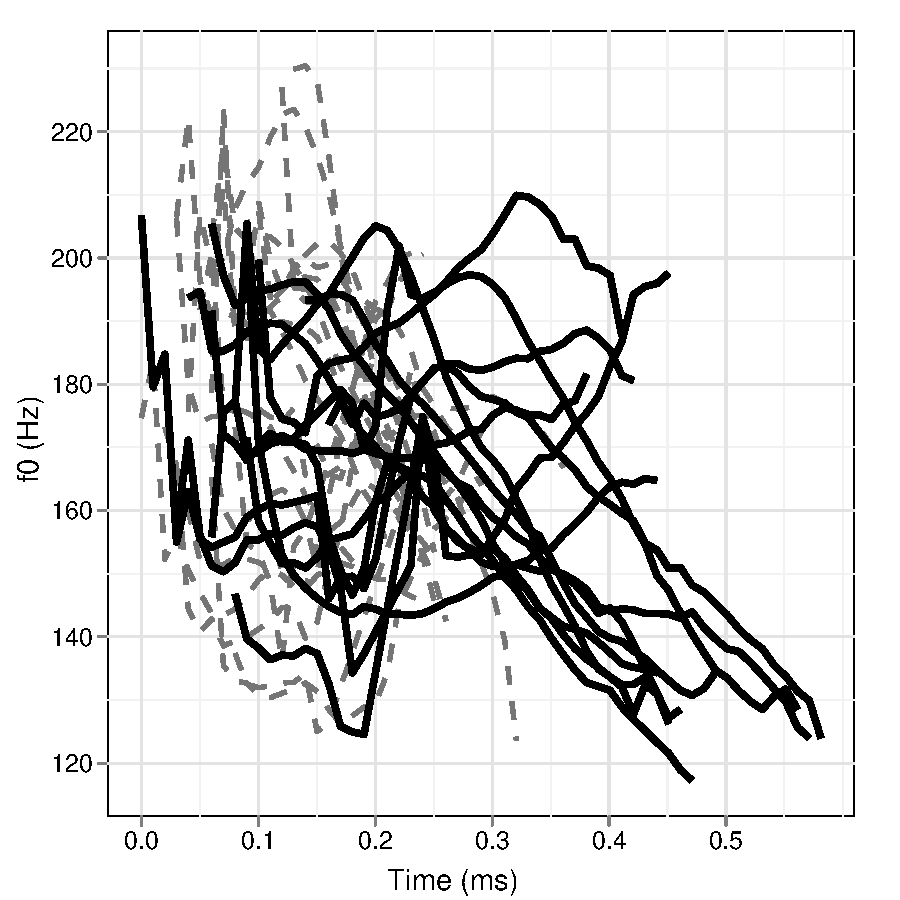
\includegraphics[width=\textwidth]{kiy-20111208-plot-iso}%
    \caption{Contours from the isolation frame drawn in black solid
      lines;
      all other contours drawn in gray dashed lines.}
    \label{fig:plot-iso}
  \end{subfigure}
  \caption{f0 contours of target words from all recorded elicitation
    items in \texttt{20111208-6-kiy-ap-nps-vps}. When the contours
    from the isolation frames are differentiated from contours from
    other frames in Figure
    \ref{fig:plot-iso}, we move some of the variability in the f0
    contours from being unexplained in
    Figure \ref{fig:plot-unexplained2} to being explained.}\label{fig:messes}
\end{figure}

If we take a closer look at the non-isolation contexts, we find that
further differentation between substitution frames in plotting f0
contours appears to reveal some additional structure in the set of f0
contours. Figure \ref{fig:plot-targets-mess} shows f0 contours from
non-isolation contexts, grouped by substitution frame. The f0 contours
from VP frames include rises, while the f0 contours from adjective
frames are falls. 

However, the relation between frame and f0 contour shape is likely
spurious. In Figure \ref{fig:plot-targets-facet}, we plot f0 contours
for each target word in separate subplots, and the f0 contours within
each subplot are very similar to one another despite being elicited in
different substitution frames. It's clear from Figure
\ref{fig:plot-targets-facet} that the structural regularity in the f0
contours we found in Figure \ref{fig:plot-targets-mess} is not due to
the effect of different substitution frames, but rather, due to the
effect of syllabic length of the target word: the f0 contours for the
monosyllabic \textit{foo} and \textit{kee} fall steeply, while the f0 contours
for the bisyllabic words show other patterns. It was an accident that
only monosyllabic target words were elicited in adjective substitution
frames. 

\begin{figure}[h]
  \centering
  \begin{subfigure}[t]{0.5\textwidth}
    \centering
    \includegraphics[width=\textwidth]{kiy-20111208-plot-targets-niso-mess}%
    \caption{Contours for all words plotted together, with frames
      indicated by line type and color.}
    \label{fig:plot-targets-mess}
  \end{subfigure}

  \begin{subfigure}[t]{0.7\textwidth}
    \centering
    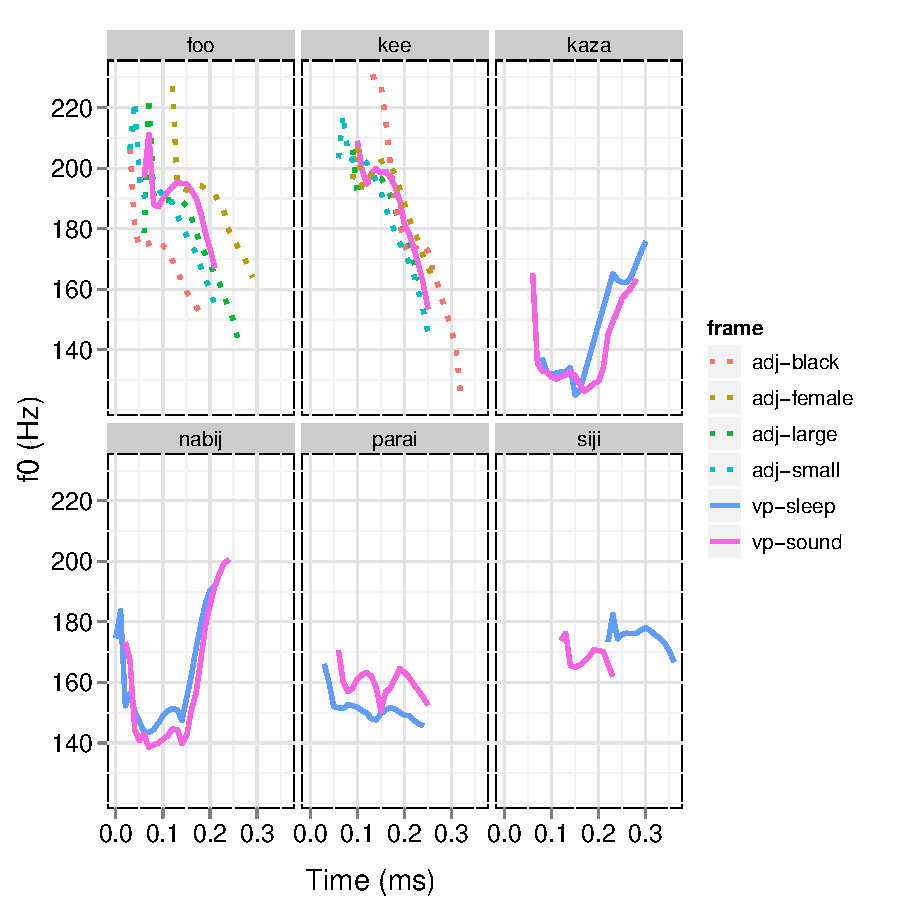
\includegraphics[width=\textwidth]{kiy-20111208-plot-targets-niso}%
    \caption{Contours plotted separately for each target word, with
      frame indicated by color and line type.}
    \label{fig:plot-targets-facet}
  \end{subfigure}
  \caption{f0 contours of the substitution items \textit{foo} `wallaby',
    \textit{kee} `ant', \textit{kaza} `gecko', \textit{nabij} `dog',
    \textit{parai} `bandicoot', and \textit{siji} `pig'  from recorded elicitation
    items in \texttt{20111208-6-kiy-ap-nps-vps}.}\label{fig:plot-targets}
\end{figure}

\clearpage

The lack of structure in the set of f0 contours in Figure
\ref{fig:plot-targets-mess} in contrast to the orderliness of the set of f0 contours plotted by
target word in Figure \ref{fig:plot-targets-facet} suggests that the
target word is a large source of variability in the pitch contour. However, the substitution frame and associated properties are not a
large source of variability, since f0 contours elicited in different
substitution frames for the same target word are very similar.      
A glance at the marked difference between f0 contours for \textit{nabij} and
\textit{parai}, despite their sharing the same
\textsc{length} adn \textsc{lexical class}, is strong evidence that we are
missing some property of the target word, some latent variable, that is a large source of
variability in the pitch contour: namely, \textsc{tonal class}. 


\subsection{Experimental design in later toneme discovery: tonemes as
  independent variables}
\label{sec:pike-toneme-design}

In \S\ref{sec:pike-toneme-early}, our explanatory variables are a
bunch of variables that we think could influence pitch contours over
words within an elicitation item and thus obscure the relation between
pitch contour variability and \textsc{tonal class} posited in
the linking hypothesis, Hypothesis \ref{hyp:link1}. Such variables are called
\textit{confounding variables}, and we performed a sleight of hand in
\S\ref{sec:pike-toneme-early} in treating these contextual variables
as if they were explanatory variables.

Once we have enough experience with tonal classes to group words by
their putative tonal classes, we can begin to treat (putative)
\textsc{tonal class} (of the target word, the substitution item) as an
\textit{independent variable} to be systematically manipulated,
alongside the set of independent variables given in Table
\ref{tab:pike-iv}. 
Our research question at this stage of toneme discovery becomes:

\begin{question}[The effect of \textsc{tonal class} on pitch contours]
\hfill\break
How does \textsc{tonal class} affect the pitch contour of a word? 
\end{question}


Asking this research question introduces a new partition in our set of
independent variables: the partition between \textit{explanatory} and
\textit{confounding} variables (also called \textit{extraneous} or
\textit{nuisance} variables). Since what we are interested in is the
effect of \textsc{tonal class} on the pitch contour, \textsc{tonal
class} is an explanatory variable. All the other independent variables
(those enumerated in Table \ref{tab:pike-iv}) are confounding
variables. In the experimental design when \textsc{tonal class} was
not yet on the table as an independent variable (\S\ref{sec:pike-toneme-early}), all
the independent variables were treated as being explanatory variables
to see if we could explain away all the variance in pitch contours
over words with them, without resorting to the latent variable of
\textsc{tonal class}. 

In this new experimental design, we treat
\textsc{tonal class} differently
from the confounding variables, as it is the sole explanatory
variable, and compare the proportion of variability explained with
\textsc{tonal class} included as an independent variable to the
proportion explained when it is not included. We deal with the confounding variables
with strategies following the classic work of \citet{Fisher:1925,Fisher:1935}.

Fisher proposed three strategies for reigning in the effect of
confounding variables on the dependent variable: blocking,
replication, and randomization.

\subsubsection{Blocking and replication}
\label{sec:blocking}

Pike's strategy of dividing elicitation items into uniform groups is
an example of \textit{blocking} confounding variables and was
conceived as such:

\begin{quote}  
\textsf{\small{In order to be significant the tonal contrasts must be
found in words which are sufficiently similar to rule out interference
from nonpitch characteristics, and they must occur in contexts which
cannot cause the observed pitch differences. \citep[p.\
48]{Pike:1948}}}
\end{quote}

For instance, elicitation items are split into homogenous groups by
the blocking variable \textsc{lexical class} of the word: one block
consists of only nouns, another block of only verbs, etc. Within each
of these blocks, the level of \textsc{lexical class} is held constant,
and each elicitation item is assigned to one level of the explanatory
variable \textsc{tonal class}, e.g.\ Tone 1. Within an elicitation
session, elicitation items are organized by these blocks: all items
within one block are elicited before moving onto the next block.\footnote{A powerful
  feature of Toney (see this volume) is to provide an easy way to
  perform post-hoc blocking, i.e.\ blocking of items from an
  elicitation session after the session is completed. Even if blocking
was not imposed during the session, Toney can extract clips of items
and play them such that one can hear all the items in a post-hoc block
one after the other.}.    All the variables in
Table \ref{tab:pike-iv} are treated as blocking variables. Although there
are multiple blocking variables, we can create a single aggregate blocking
variable called \textsc{block} subsuming all the
confounding variables in Table \ref{tab:pike-iv}.\footnote{There are
  more sophisticated ways to incorporate multiple blocking variables
  into an experimental design, such as the Latin square designs
  commonly used in psycholinguistics
  \citep[p.\ 136--142]{Montgomery:2005}, but
  it's sufficient for our purposes here to conceptually discuss a single aggregate
  blocking variable.} Thus, a block
consists of a homogenous group of elicitation items, matched for every
variable listed in Table \ref{tab:pike-iv}, e.g.\ one level of the
\textsc{block} variable might be the group of items
specified by the fixed levels in Table \ref{tab:pike-block}. This is
like a generalized substitution frame, a complete fixed aggregate
specification of context for an elicitation item.

Let's expand on this notion of a generalized substitution frame:
while Pike refers to only the substitution frame as ``context'' in the
quote about blocking above, we extend ``context'' to refer to the
morphophonological properties of the words from the first step in the
procedure as well: since we would like to assume that any variation in
pitch patterns between words is due solely to tonemic contrast,
\textit{any} aspect of the elicitation situation that affects the
pitch of a word, but which isn't tonal class, is part of the
``context''. What is of primary scientific interest here is tonemic
contrast as the source of pitch variation between words. Thus, we make
the methodological abstraction of setting aside sources, other than
tonal class, that would potentially generate pitch variation between
words.\footnote{The strategy of making methodological abstractions in
the process of groping toward scientific understanding---setting
contextual factors aside (for the moment) to hone in on what is of
primary interest---is an old one. \citet{Plato:360} described it as
carving nature at its joints.}
 

\begin{table}[!h]
  \centering
  \begin{tabular}{l | l}
    Variable & Fixed levels\\\hline
    Lexical class &  noun\\
    Morphological complexity &  simplex\\
    Syllabic length & disyllabic\\
    CV skeleton &  CVCV\\
    (Vowel length) &  (short)\\
    Segmental features &  initial voiceless obstruent\\\hline
    Prosodic position &  utterance-initial\\
    Pragmatic context &  Out of blue focus\\
    Syntactic structure &  Possessive prenominal phrase\\
  \end{tabular}
  \caption{An example of a block specification aggregated over the
    confounding variables in Table \ref{tab:pike-iv}. Each of the
    confounding variables are fixed at the levels stated in the
    table, e.g.\ \textsc{lexical class} in the block is fixed to be ``noun''. We might call
    this particular specification of the confounding variables \textit{Block 1}, one of multiple levels of the aggregate
    blocking variable \textsc{block}. Another block, say \textit{Block
    2}, might have identical specifications other than that
  \textsc{lexical class} is ``verb'' rather than ``noun''  in \textit{Block 2}.}
  \label{tab:pike-block}
\end{table}

By blocking, we can take advantage of our knowledge of some of the
sources of variability in the pitch contour of a word. Rather than
leaving the variability induced by those sources as unexplained, we
parcel that variability out between blocks, i.e., as variability explained
by the blocking variable, thus adding to the proportion of variability
explained. Previously, when we treated \textsc{tonal class} as a
latent variable, explained variability consisted only of variability
explained by variables aggregated in \textsc{block}. Now, the explained variability consists of variability
explained by \textsc{tonal class} as well as variability explained by
variables aggregated in \textsc{block}. 

Blocking reduces the noise in the
observed effect of \textsc{tonal class} on pitch contours. Across
blocks, the effects of \textsc{tonal class} on pitch contours might
look quite different, so that the
particular pitch contours induced over words by different tonal
classes may be quite different. But within a
homogeneous block, systematic variability in pitch contour induced by
\textsc{tonal class} is much clearer since variability in pitch
contours within a block due to factors other than \textsc{tonal class} is
small. What is uniform across blocks is not the particular pitch
contours induced by a given tonal class, but the unified, group
behavior of members of a tonal class within each block in patterning
as a unit. 

An
additional benefit of blocking is that each block serves as a
\textit{replication} of the experiment testing to confirm the way that
\textsc{tonal class} affects pitch contours of target
words. Converging evidence from each replication about systematic
variability in pitch contours due to tone classes boosts our
confidence about our posited tonal contrasts. 

However, sometimes
fixing a confounding variable at a constant level for the whole
experiment, i.e. running just a single block, is also a good
option. (Sometimes one can also run just a subset of multiple levels among all the
possible levels, but this is less common than running either all of
the levels or just one, since it's hard to justify why one picked some levels
but not others.) 

For instance, one might consider the variable \textsc{sonorancy} (of all
consonantal segments in the target word), with the
two levels [+sonorant], [-sonorant]. One could vary between these two
levels between blocks, but one could also fix \textsc{sonorancy} to be
[+sonorant]. This is very common in intonational experiments, since
working exclusively with [+sonorant] segments can help reduce
segmental perturbations to the pitch contour when tone-segment
interactions are not of interest (see
\S\ref{sec:pitch-tracking}). Abstracting away from [-sonorant]
consonants has the disadvantages that we miss the opportunity to: (1) replicate our elicitation experiment to build our confidence in our
conclusions about toneme discovery, and (2) study interactions
between levels of \textsc{sonorancy} and \textsc{tonal class}. But by
fixing \textsc{sonorancy} at [+sonorant], we have the advantages of:
(1) reducing noise in the relation between \textsc{tonal class} and
the pitch contour, thus making it easier to uncover tonemes, and (2)
reducing the number of items in the elicitation so that the
elicitation isn't too long and grueling. 

Whether it's best to hold a
confounding variable fixed or to vary it depends entirely on the research
question. We provide some examples of making this decision in
\S\ref{sec:generalize-exp-design} and \S\ref{sec:gen-question}, but
it's really a case-by-case decision so it's difficult to give general
guidelines. One rule of thumb for factors to consider in the decision,
if there are no other compelling reasons based on the research
question, is to consider either choosing the ``vanilla'' level or
choosing one or more extreme levels.\footnote{Thank you to Pat
  Keating for teaching me this.} By ``vanilla'' level, we mean,
roughly speaking, the most unmarked level. For instance, for
\textsc{syllable structure}, this might be CV rather than CCV, CVV, or
CVC, depending on the word-prosody of a language. Picking a
``vanilla'' level can be a good option when you are wholly uninterested
in the variable and simply need to choose something in order to set up
your experiment. Picking extreme
levels can be a good option when you are more interested in the
interaction between your explanatory variable(s) and the confounding
variable at hand---perhaps you're worried about generalizing your
conclusions across the levels of the confounding variable, so
performing replications at one or more extreme levels provides
converging evidence for your conclusions and/or a challenging test of your
hypotheses under worst case limiting conditions.\footnote{The
  strategy of testing extreme cases is common for error checking and
  debugging in mathematics and programming, too.}

\subsubsection{Randomization}
\label{sec:randomization}

Some confounding variables are not amenable to blocking. Consider the
order of elicitation items:

\begin{quote}  
\textsf{\small{The mere fact that one word is necessarily said before the
  other in repetitions by the informant will frequently cause
  sandhi changes, or phrasal conditioning, or intonational
  modifications of one of the words. To check on this possibility
  the investigator should (1) reverse the order in which the
  items are repeated, and (2) have the informant make a marked
  pause before each item. \citep[p.\ 54]{Pike:1948}}}
\end{quote}

As Pike states, it is unavoidable that the elicitation context sets up
a discourse context in which the discourse extends beyond single
elicitation items. Thus, prosodic marking of prominence and
demarcation (phrasing) due to the imposition of prosodic structure
and/or the particular pragmatic context introduced in the current
discourse context may induce variation in pitch contours. Particularly
dire is if there is a bias in where elicitation items of a given tonal
class appear in the order of items. Suppose that the tonemes of a tone
language include a falling tone as well as a low tone. Now suppose
that within each block, we have one item exemplifying each toneme, and
that the low tone items are always elicited at the
end of the block. Since low tones often fall utterance-finally due to
the interaction of tonal and intonational effects on the pitch
contour, we might not be able to distinguish the true falling tone and
the low tone.  

 What would be the levels of an independent variable \textsc{order}
 (of tonal class)? Suppose we had five tonal classes, and one exemplar of each
tone class to use as a substitution item within a block such as the
block specified in Table \ref{tab:pike-block}. With only five items, we
would have 5! = 5 * 4 * 3* 2 * 1 = 120 possible orders of the items within the block!
Adding elicitation order as a blocking variable would add 120 times as
many blocks. Another problem with blocking by \textsc{order} is that it's
not clear that this is the way we would want to define elicitation
order---perhaps all that matters is what \textsc{tonal class} level is last in a
block. Then we would only have five levels of \textsc{order}, one
level for each of the five elicitation items occupying the last slot in
the block. Or alternatively, perhaps what matters is the identity of
the \textsc{tonal class} of two elicitation items that occur next to one another in the elicitation
sequence.  

An alternative to blocking is \textit{randomization}:

\begin{quote}
\textsf{\small{Randomisation properly carried out $\ldots$ relieves the experimenter from the anxiety
of considering and estimating the magnitude of the innumerable causes
by which his data may be disturbed. \citep[p.\ 44]{Fisher:1935}}}
\end{quote}

Rather than blocking by \textsc{order}, rather than attempting to make
sure that there are no biases in ordering with respect to
\textsc{tonal class} by painstakingly fiddling with orders by hand, we
\textit{randomize} order of elicitation items within a block to
eliminate bias. One way to conceptualize this is the following: for
each block, suppose we label each elicitation item within that block
with an integer, e.g.\ 1, 2, 3, $\ldots$, 24, 25 if there are 25 items
in the block. We then write that number on a slip of paper and put all
of the slips in a jar and mix them up. Each time we're ready to elicit
a new item within a block, we draw a slip from the jar and read the
number written on it. The number on the slip tells us which item to
elicit. We then put the slip in the recycling bin (not back in the
jar) and elicit the corresponding item. 

This concludes our discussion of the second stage in toneme discovery,
where (putative) \textsc{tonal class} is treated as an independent
variable. In \S\ref{sec:kiy-iv} below, we illustrate an example of
manipulating \textsc{tonal class} as an independent variable in
Kirikiri, focusing on blocking and replication as strategies. In the
tutorial [SEE TUTORIAL], we show ways to perform simple randomizations of
elicitation order with examples from Kirikiri elicitations.

\subsubsection{Example: \textsc{tonal class} as an independent variable in
Kirikiri}
\label{sec:kiy-iv}

In \S\ref{sec:example-latent-kiy}, we gave an example of discovering
\textsc{tonal class} as a latent source of variability in the pitch
contour in Kirikiri. In this section, we fast forward a bit to one of
the first elicitation sessions where we explicitly treated
\textsc{tonal class} as an independent variable and systematically ran
exemplars of different proposed tonal classes through a series of
substitution frames in $N_1 N_2$ prenominal possessive
constructions. This is elicitation session
\texttt{20111213-kiy-ap-1-framedwordlist}.

The substitution frames are chosen to treat
\textsc{tonal class} of the substitution frame, a single word, as a
blocking variable, so each of the five proposed tonal classes for the
substitution frame serve as a block for replication for testing the
proposed tonal classes of the substitution items (target words). In
fact, the experimental design has two experiments in one: we can consider
either $N_1$ to be the substitution item and $N_2$ to be the
substitution frame, or vice versa. When the target word is $N_1$, it's
utterance-initial, and when it is $N_2$, it is utterance-final, so we
have experimental replications over different prosodic positions, as
well as replications over different flanking tonal classes. The experimental design for this
session, taking $N_1$ to be the substitution item is given below. The
experimental design taking $N_2$ to be the substitution item is nearly
identical: wherever $N_1$ occurs in the description of the
experimental design, replace it with $N_2$.

\begin{itemize}
  \item Research question: How does \textsc{tonal class} affect pitch
    contour over a word?
  \item Strategy: Manipulate \textsc{tonal class} as an independent
    variable in different substitution frames. 
  \item Research hypothesis: There are five tonal classes in Kirikiri.
  \item Linking hypothesis: We assume that distinct pitch contours
    imply distinct levels of \textsc{tonal class}, as in Hypothesis
    \ref{hyp:link1}. Moreover, we assume that in one or more substitution frames, the
    pitch contour for a proposed tonal class is distinct from pitch
    contours for other proposed tonal classes.
  \item Experimental unit: individual elicitation items
  \item Explanatory variables: \textsc{tonal class} (of target word $N_1$), with levels $T1$, $T2$, $T3$,
  $T4$, $T5$
  \item Confounding variables
  \begin{itemize}
    \item \textsc{word length} (of target word, in syllables): 2 syllables (fixed at this
    level)
    \item \textsc{syntactic structure}: prenominal possessive phrases (fixed)  
    \item \textsc{tonal class of frame word} $N_2$, with levels $T1$, $T2$, $T3$,
  $T4$, $T5$ $\ldots$ (blocking variable)
    \item \textsc{prosodic position} (of substitution item):
      utterance-initial (fixed; utterance-final if $N_2$ is the target
      word)
    \item \textsc{word length} (of substitution frame in syllables): 2
      syllables (fixed)
  \end{itemize}
  \item Dependent variable: pitch contour over the target word $N_1$
\end{itemize}

A list of the five different blocks for each of the two
sub-experiments, one with $N_1$ as the target word, and one with $N_2$
as the target word, is given in Table
\ref{tab:kiy-20111213-bigrams}. The full layout of tonal sequences in
the experimental design is given in Table \ref{tab:factorial-kiy}. The
levels of the independent variables $N_1$ \textsc{tone} and $N_2$
\textsc{tone} are fully cross-classified. We'll see another way to
think about these kinds of fully cross-classified designs in
\S\ref{sec:tonotactics}. The exemplar words chosen for each
\textsc{tonal class} for $N_1$ and $N_2$ are given in Table
\ref{tab:kiy-wordbank}.

\begin{table}[!h]
  \centering
  \begin{tabular}{l | c c}
    Block & IV  & Levels\\\hline
    $N_2$: T1 & $N_1$ \textsc{tone} & T1, T2, T3, T4, T5\\
    $N_2$: T2 & $N_1$ \textsc{tone} & T1, T2, T3, T4, T5\\
    $N_2$: T3 & $N_1$ \textsc{tone} & T1, T2, T3, T4, T5\\
    $N_2$: T4 & $N_1$ \textsc{tone} & T1, T2, T3, T4, T5\\
    $N_2$: T5 & $N_1$ \textsc{tone} & T1, T2, T3, T4, T5\\\hline
    $N_1$: T1 & $N_2$ \textsc{tone} & T1, T2, T3, T4, T5\\
    $N_1$: T2 & $N_2$ \textsc{tone} & T1, T2, T3, T4, T5\\
    $N_1$: T3 & $N_2$ \textsc{tone} & T1, T2, T3, T4, T5\\
    $N_1$: T4 & $N_2$ \textsc{tone} & T1, T2, T3, T4, T5\\
    $N_1$: T5 & $N_2$ \textsc{tone} & T1, T2, T3, T4, T5\\
  \end{tabular}
  \caption{Manipulated independent variables (IVs) in the experimental
    design for elicitation session
    \texttt{20111213-1-kiy-ap-framedwordlist}. \textsc{tonal class}
    for $N_1$ ($N_2$), the target word, is varied over the 5 putative tonal
    classes within each block of varying the tonal class of the
    substitution frame word, $N_2$ ($N_1$). }
  \label{tab:kiy-20111213-bigrams}
\end{table}


\begin{table}[!h]
  \centering
  \begin{tabular}{l | l l l l l}
     & +\textit{T1} & +\textit{T2} & +\textit{T3} & +\textit{T4} & +\textit{T5} \\\hline
     T1 & T1 + T1 & T1 + T2 & T1 + T3 & T1 + T4 & T1 + T5\\
     T2 & T2 + T1 & T2 + T2 & T2 + T3 & T2 + T4 & T2 + T5\\
     T3 & T3 + T3 & T3 + T2 & T3 + T3 & T3 + T4 & T3 + T5\\
     T4 & T4 + T1 & T4 + T2 & T4 + T3 & T4 + T4 & T4 + T5\\
     T5 & T5 + T1 & T5 + T2 & T5 + T3 & T5 + T4 & T5 + T5\\
  \end{tabular}
  \caption{Manipulation of \textsc{tonal class} as an independent
    variable in a sequence of two tones. The levels of the independent
    variables  $N_1$
    \textsc{tone} and $N_2$ \textsc{tone} are cross-classified
    so that all possible combinations of tones ($5 \times 5 = 25$ in
    total) are included.}
  \label{tab:factorial-kiy}
\end{table}

\begin{table}[!h]
  \centering
  \begin{tabular}{c | c l}
    Tone& Noun & Word \\\hline
    T1 & N1 & parai `bandicoot'\\
     & N2 & giru `elbow'\\\hline
    T2 & N1 & kaza `gecko'\\
     & N2 & ora `tongue'\\\hline
    T3 & N1 & fivaa `snail'\\
     & N2 & faro `groin'\\\hline
    T4 & N1 & naraa `wasp'\\
     & N2 & kwawaa `chin'\\\hline
    T5 & N1 & tava `catfish'\\
     & N2 & koree `string'\\\hline
  \end{tabular}
  \caption{Wordbank for $N_1+N_2$ data set from \texttt{20111213-1-kiy-ap-framedwordlist}}
  \label{tab:kiy-wordbank}
\end{table}

In Figure \ref{fig:20111213-plot-all-by-tone}, we show f0 contours for
all words, whether they were utterance-initial ($N_1$) or
utterance-final ($N_2$). All f0 contours plotted in this section are
\textit{time-normalized}. For each f0 contour, mean f0 was extracted from 30 evenly
spaced frames over the word, so, for instance. The effect of this normalization is to
improve comparability of the shape of f0 contours over words that may
have different durations and/or have been uttered at different speech
rates. When we differentiate the f0 contours by \textsc{tonal class},
it is clear that there is structure in the mess of f0 contours shown
in the plot. 

\begin{figure}
  \centering
  \includegraphics[width=0.8\textwidth]{kiy-20111213-plot-all-by-tone}
  \caption{A plot of time-normalized f0 contours from all target words elicited in the session
    \texttt{20111213-1-kiy-ap-framedwordlist} for both $N_1$ and $N_2$. Tone class is indicated
  by color and line type. The x-axis indicates \textit{samples}, not
  an absolute time scale since the f0 contours are
  time-normalized. For each word, 30 evenly spaced samples were taken
  from the f0 contour. }
  \label{fig:20111213-plot-all-by-tone}
\end{figure}

When we separately plot time-normalized f0 contours for $N_1$ and
$N_2$, see Figures \ref{fig:kiy-20111213-plot-w1} and
\ref{fig:kiy-20111213-plot-w2}, the huge effect that \textsc{tonal class}
has on variability in the f0 contour is quite apparent. Even though we
haven't separated f0 contours by \textsc{substitution frame}, the
contours within each tonal class in each figure have very similar shapes and pitch
ranges. However, the f0 contours for the same \textsc{tonal class}
across substitution frames can be quite different. For instance, T2 in
$N_1$ shows a large fall at the end of the word, but the same tone in
$N_2$ has have a large pitch rise to the end of the word, and T3 in
$N_1$ has a large early peak, while T3 in $N_2$ has no large peak.

\begin{figure}
\centering
\begin{subfigure}[t]{0.5\textwidth}
  \centering
  \includegraphics[width=\textwidth]{kiy-20111213-plot-w1}
  \caption{Time-normalized f0 contours for $N_1$ only.}
  \label{fig:kiy-20111213-plot-w1}
\end{subfigure}

\begin{subfigure}[t]{0.5\textwidth}
  \centering
  \includegraphics[width=\textwidth]{kiy-20111213-plot-w2}
  \caption{Time-normalized f0 contours for $N_2$ only.}
  \label{fig:kiy-20111213-plot-w2}
\end{subfigure}
\caption{Time-normalized f0 contours plotted separately for $N_1$ and $N_2$.}\label{fig:w1w2}
\end{figure}

Finally, Figures \ref{fig:kiy-20111213-plot-w1-facet} and
\ref{fig:kiy-20111213-plot-w2-facet} emphasize just how much variability in
the pitch contour over the word can be attributed to \textsc{tonal
  class}. Within each tonal class, f0 contours for $N_1$  or $N_2$ are
remarkably similar.

\begin{figure}
\centering
\begin{subfigure}[t]{0.5\textwidth}
  \centering
  \includegraphics[width=\textwidth]{kiy-20111213-plot-w1-facet}
  \caption{f0 contours for $N_1$ by tonal class}
  \label{fig:kiy-20111213-plot-w1-facet}
\end{subfigure}

\begin{subfigure}[t]{0.5\textwidth}
  \centering
  \includegraphics[width=\textwidth]{kiy-20111213-plot-w2-facet}
  \caption{f0 contours for $N_2$ by tonal class}
  \label{fig:kiy-20111213-plot-w2-facet}
\end{subfigure}
\caption{Time-normalized f0 contours plotted separately for $N_1$ and
  $N_2$ for each putative tonal class.}\label{fig:w1w2-facet}
\end{figure}


\clearpage

\section{Using experimental design principles to generalize beyond
  Pike (1984)}
\label{sec:generalize-exp-design}

In \S\ref{sec:pike-toneme-early} and \S\ref{sec:pike-toneme-design},
we've seen how Pike's toneme discovery procedure can be recast in
terms of general principles of experimental design. In this section,
we show how understanding Pike's procedure in terms of experimental
design allows us to relate Pike's elicitation methodology to other
methods in tonal elicitation, via: (1) applying the same principles to
a different set of variables
(\S\ref{sec:gen-iv}), including the special case
of considering alternative ways of defining variables within Pike's
procedure (\S\ref{sec:gen-param}), and (2) applying the same
principles to different research questions (\S\ref{sec:gen-question}).

\subsection{Generalizing the set of independent variables}
\label{sec:gen-iv}

One simple generalization beyond Pike's procedure is the consideration
of additional independent and dependent variables.  If we keep our research question
about toneme discovery, then any additional independent variables must all be
confounding variables, since our only explanatory variable is
\textsc{tonal class} for toneme discovery. Measuring additional dependent
variables for toneme discovery presupposes additional linking
hypotheses between tonemes and phonetic parameters, such as aspects of
voice quality like parameters indexing creakiness and breathiness. We
consider such dependent variables beyond pitch, as well as pitch-based
variables, in \S\ref{sec:pitch}. In this section, we focus on expanding the set
of independent variables considered.

Another independent variable is \textsc{elicitation
session}. Sometimes speakers may produce different pitch contours for
the same target word in the same context (as captured by our set of
confounding variables) from elicitation session to elicitation
session. Perhaps the consultant was tired during one of the sessions
and misunderstood what was intended to be elicited; perhaps
intervening sessions affected the discourse context of the elicitation
session--who knows? Some sources of variability in pitch contour
generation we might never be able to get a grip on, but we may still
move some variability from the \textit{unexplained} partition to the \textit{explained}
variability partition by blocking by aggregate confounding variables like
\textsc{elicitation session}. \textsc{elicitation session} acts as a
cover term for the factors in play that vary over time between
elicitation sessions, and by repeating elicitations across sessions,
we add additional replication into the experimental design. 

We enumerate some other potential confounding variables within a subject for the effect of
\textsc{tonal class} on pitch contours over a word in Table
\ref{tab:confounds}. We provide a couple of example
levels for each variable, as well as sample references which either manipulated the
variable or discuss the relation between the variable and variability
in the pitch contour. The listed confounds range
from physiological factors to phonological and morphosyntactic
grammatical factors to discourse and pragmatic factors. 

It may seem
counterintuitive to consider grammatical factors such as
\textsc{case} to be confounding, since the underlying source of pitch
variability is grammatical tone marking. But if the research question
is to uncover how tonemic contrast---how \textit{lexical} \textsc{tone class}---affects the
pitch contour, then grammatical tone marking is indeed a
confound. Take case-marking in Maasai (Kenya), e.g.\ \`end\'er\`on\`i
`rat.\textsc{nom}' and \`end\`er\'on\`i `rat.\textsc{acc}'
\citep[p.\ 203]{Hyman:2011b}. Suppose you had been eliciting simple
determiner phrases, by coincidence in nominative case, e.g.\ in
isolation or in response to ``What saw the man?'',  and mixed in
determiner phrases in accusative case in the same block---without
including \textsc{case} as a confounding variable---e.g.\ in
response to the question ``What did the man see?''. In that case, the
variability between \`end\'er\`on\`i
`rat.\textsc{nom}' and \`end\`er\'on\`i `rat.\textsc{acc}' would be
bundled into unexplained variability and cloud the relation between
the putative toneme sequence LHLL and the pitch contour over the word. If one
were instead investigating the relation between \textsc{case} and the
pitch contour over the word, then \textsc{tone class} would
be a confound. What is an explanatory variable and what is a
confounding variable always depends on the research question. To abuse
the old saw about junk and treasure,
``one experiment's confounding variable is another experiment's explanatory variable.''

\begin{table}[!h]
  \centering
  \begin{tabular}{p{1.5in} | p{1.8in} p{2.4in}}
    Variable & Example levels & Reference\\\hline
    Speech rate &  slow, fast & \citet{Fougeron:1998,Gandour:1999,Kuo:2007} \\
    Speaker pitch range & small, large & \citet[p.\ 175]{Baken:2000}
    \\
    Background noise & absent, present & \citet{Zhao:2009} \\
    Consonant voicing &  Voiced, unvoiced  & \citet{Hombert:1978} \\
    Vowel quality &  High, low & \citet{Connell:2002,Hombert:1978}\\
    Prosodic position  & Utterance-final, phrase-medial  & \citet[p.\
    45-46]{Maddieson:1978}, \cite{Hayes:1989}, \cite{Shattuck-Hufnagel:1996}, \citet{Zsiga:2007}, \cite[Ch.\ 6]{Gussenhoven:2004} \\
    Declination  & Phrase-initial, phrase-final & \cite[Ch.\ 6]{Gussenhoven:2004} \\
    Downstep & Post-trigger & \cite[Ch.\ 6]{Gussenhoven:2004} \\
    Tonal coarticulation and sandhi  & preceding H, following L
    & \citet{Xu:1997a,Chen:2000,Kuo:2007}  \\
    Lexical frequency  & low, high & \citet{Zhao:2009} \\
    Person & 1sg, 3sg  & \citet[p.\ 203]{Hyman:2011b} \\
    Tense/aspect  & present, past  & \citet[p.\ 203]{Hyman:2011b} \\
    Negation  & present, absent  & \citet[p.\ 203]{Hyman:2011b} \\
    Case  & nominative, accusative & \citet[p.\ 203]{Hyman:2011b}\\
    Emphasis level  & 1 (mumble), 10 (shout)  &
    \citet{Liberman:1984}\\
    Focus & Contrastive focus, out-of-blue focus  &
    \citet{Katz:2011}, \citet{Eady:1986}, \citet{Jun:2005}\\
    Giveness  & Given, new  &
    \citet{Katz:2011}\\
    Speech style  & spontaneous, reading &
    \citet{fernald:1984}, \citet[p.\ 175-176]{Baken:2000}\\
    Phonetic accommodation  & pre-exposure, post-exposure  & \citet{Babel:2012,Babel:2012a}\\
%    Repetition & Lexical & low, high & \citet{Zhao:2007} \\
  \end{tabular}
  \caption{Some additional examples of potential confounding variables in
    toneme discovery, arranged roughly in order from variables related
    to: physiology and the speech signal, phonetics and phonology,
    morphosyntax, and discourse and pragmatics.}
  \label{tab:confounds}
\end{table}


% OIL OIL OIL
% \subsubsection{Example: mysterious session-to-session variability in Kirikiri}
% \label{sec:kiy-variability}


% \subsubsection{Example: repetition in Kirikiri}
% \label{sec:kiy-rep}

% Repetition vs. replication??

% \subsubsection{Example: formality and voice quality in Igbo}
% \label{sec:igbo}

% \subsubsection{Example: rapport?? in Samoan? style?}
% \label{sec:igbo}


% \subsubsection{Example: Yoruba grammar as confound}
% \label{sec:yoruba}

% \subsubsection{Example: Bole H tone spreading as confound}
% \label{sec:yoruba}

% \subsubsection{Example: Vowel height-tone interactions in Kirikiri}
% \label{sec:vowel-height}


\subsection{Parametrizing variables}
\label{sec:gen-param}

A special case of generalizing the set of variables under
consideration (\S\ref{sec:gen-iv}) is when we don't add any new variables, but
we change the definition of some of the variables. There are two main
ways in which we might do this:

\begin{itemize}
  \item Coarsening the partition of the possible instantiations of the
  variable
  \item Refining the partition of the possible instantiations of the
  variable
\end{itemize}

When we coarsen the partition, we reduce the number of levels for a
variable, merging levels with one another. When we refine the
partition, we increase the number of levels for a variable, splitting
levels. 

One example of coarsening the partition is given in Table
\ref{tab:tonal-class}. This is adapted from the study of contextual
tonal variation in Mandarin in \cite[p.\ 70]{Xu:1997a}. The
explanatory variable of \textsc{tonal class} of the target syllable
had 4 levels, following the 4-way tonal contrast in Mandarin
(abstracting away from the neutral fifth tone). However, the
explanatory variable of the \textsc{pre-target tone}, i.e.\ the tone
class of the syllable preceding the target syllable, collapsed the
4-way distinction for Mandarin tonal classes into a 2-way distinction
based on the tonal offset: both Tone 1, a high tone, and Tone 2, a
rise, were classified as having a high offset, and both Tone 3 (low) and
4 (fall) were classified as having a low offset. In
autosegmental-theoretic terms  \citep{Goldsmith:1990,Goldsmith:1976},
one might say that the new variable assumes that contour tones are treated as tonal
sequences (fall = HL, rise = LH) and pays attention only to the tone at the
right edge of the syllable.  

\begin{table}[!h]
  \centering
  \begin{tabular}{l | l l l}
    Tone & Old level & Mapping & New level\\\hline
    Tone 1 & High & High $\mapsto$ H & H\\
    Tone 2 & Rise  & Rise $\mapsto$ H & H\\
    Tone 3 & Low & Low $\mapsto$ L & L\\
    Tone 4 & Fall  & Fall $\mapsto$ L & L\\
  \end{tabular}
  \caption{A coarsening of the levels for \textsc{tonal class} in
    Mandarin from \citet{Xu:1997a}.}
  \label{tab:tonal-class}
\end{table}

Another example of coarsening the partition defined by a variable
comes from \citet{Keating:2011}, a cross-linguistic study of the
acoustic parameters involved in distinguishing phonation types. Here,
for the purposes of standardization for comparison with other languages, the 7-way tonal
contrast in the White Hmong data from \citet{Esposito:2009, Esposito:2012} was coarsened into a 3-way contrast capturing
the rough location of the tone within the pitch range---either high,
mid, or low---for the same data, for the purposes of the cross-linguistic comparison
in \citet{Keating:2011}, see Table \ref{tab:hmong-tones}. 

\begin{table}[h]
  \centering
  \begin{tabular}{l | c c c}
    Tone & Old level & Mapping & New level\\\hline
    b-tone & High-rising & High-rising $\mapsto$ H & H  \\
    null-tone & Mid & Mid $\mapsto$ M & M  \\
    s-tone & Low & Low $\mapsto$ L & L \\
    j-tone & High-falling & High-falling $\mapsto$ H &H \\
    v-tone & Mid-rising & Mid-rising $\mapsto$ M & M\\
    m-tone & Low-falling & Low-falling $\mapsto$ L & L   \\
    g-tone & Mid-falling & Mid-falling  $\mapsto$ M & M\\
  \end{tabular}
  \caption{Coarsening of levels for \textsc{tonal class} in White Hmong. Note: the g-tone is
    high-falling for females, but we abstract away from that here. Old
    levels come from \citet{Esposito:2009,Esposito:2012}. New levels
    come from
    cross-linguistic study of phonation contrasts in \citet{Keating:2011}}
  \label{tab:hmong-tones}
\end{table}

An example of refinement of the partition induced by a variable would
be the reverse of the mapping for Mandarin tones in Table
\ref{tab:tonal-class}: rather than collapsing a 4-way distinction into
a 2-way distinction, one would refine a 2-way distinction into a 4-way
distinction. Another instance of refinement would be the addition of a
level for \textsc{tonal class} upon the discovery of 
evidence for a new tonal class in the course of fieldwork. 

Those two examples of refinement both involve increasing the number of
levels to some finite number, but refinements may also involve
mapping from a set of a finite number of distinctions, e.g.\ 4
levels, to a set of potentially infinitely many distinctions, i.e.\
the set of \textit{real numbers}.\footnote{The set of \textit{real
    numbers} contains numbers like 3.0, 1.542, $\pi$, 2.9, 2.99, 2.999,
  2.9999999999999999$\ldots$.} An
example of this kind of refinement would be changing a \textsc{length}
variable from counting syllables, e.g.\ 1 syllable, 2 syllables
$\ldots$, to measuring absolute time, e.g.\ 343.25 milliseconds,
692.11 milliseconds. This kind of refinement might seem intuitively more
drastic than refining a 2-way tonal distinction into a 4-way one, and
it is: it's a change in variable type \citep{Stevens:1937}, similar to a
change in type in type-theoretical semantics \citep[Ch.\
4]{Gamut:1992},\citep[Chs.\ 2, 3]{Carpenter:1997}. 

%dichotomous variables -> continuous (BAAYEN)

\subsection{Generalizing to different research questions}
\label{sec:gen-question}

A more drastic way to generalize beyond Pike's procedure is to apply
principles of experimental design to other research questions. In this
section, we give examples of research questions: (1) treating tone as a
dependent variable rather than an independent variable
(\S\ref{sec:tone-dv}), (2) exploring the mapping from underlying tonemes
to surface tones in Thlantlang Lai as described in \citet{Hyman:2007}
(\S\ref{sec:tonotactics}), (3) examining phonetic tonal sandhi, i.e.\
tonal coarticulation in White Hmong (\S\ref{sec:hmong}), and (4) uncovering
evidence for a tonal case marker in Samoan (\S\ref{sec:samoan-abs}). 
 

\subsubsection{Example: tone as a dependent variable}
\label{sec:tone-dv}

Thus far in this paper, we've considered \textsc{tonal class} as an independent
variable manipulated by the fieldworker, but we've never considered
\textsc{tonal class} as a dependent variable. This is not because
\textsc{tonal class} cannot be treated as a dependent variable, but
simply due to the nature of our research questions---we've focused
on making hypotheses about possible \textsc{tonal classes} and their
reflexes in the pitch contour and refining these hypotheses. 

There are two main situations in which tone might appear in the dependent
variable: 

\begin{itemize}
  \item in explorations of how tonal contrast is produced and perceived
  \item in explorations of phonological allophony and alternation 
\end{itemize}

Some example research questions about exploring the dimensions of
tonal contrast are:

\begin{itemize}
\item What effect does \textsc{tonal class} have on the pitch contour over a
word? 
\item What parameters in the speech signal are available for discriminating
different tonal classes?
\item What cues in the speech signal do listeners use to identify tones?
\end{itemize}

Some examples of work along these lines appear in \citet{Connell:2000}
(perception), \citet{Khouw:2007} (perception), and \citet{DiCanio:2009} (production).

In explorations of phonological allophony and alternation, tone makes
an appearance in the dependent variable because the mapping
between underlying tonemes and surface tones (or between surface tones) is of primary
importance. \textsc{Underlying form} is manipulated as an
explanatory variable, and the dependent variable is the surface
form. Note that there must be a linking hypothesis about the mapping
from observables (perhaps the pitch contour over a word) to surface
tones in such an elicitation experiment. We present an example of the
tonal fieldwork exploring phonological allophony in the next section, \S\ref{sec:tonotactics}.

\subsubsection{Example: tonotactics in Thlantlang Lai \citep{Hyman:2007}}
\label{sec:tonotactics}

 In
tonal fieldwork, as soon as the fieldworker is far along enough in toneme
discovery to manipulate \textsc{tonal class} as an explanatory
independent variable, a natural set of follow-up
research questions is to pursue further detail in understanding tonal
allophony and alternation. Here, we take \citet{Hyman:2007}'s work on
Thlantlang Lai (Tibeto-Burman Kuki-Chin, Myanmar) tonal allophony as an example. \citet{Hyman:2007}
examined the surface tone sequences of prenominal possessive phrases,
e.g.\ r\^{a}al r\`ang `enemy's horse'. 

We can cast this in terms of the following experiment:

\begin{itemize}
  \item Research question: Are there tonotactic $n$-gram restrictions in
  Thlantlang Lai?\footnote{An $n$-\textit{gram} is a sequence of
    discrete units of length $n$, e.g.\ a $2$-\textit{gram} or \textit{bigram}
    is a sequence of length 2.}
  \item Strategy: Control any variables suspected to induce variation in
  surface realization of underlying tones. (Tonotactic restrictions,
  perhaps formulated as constraints,
  are not included in this set of variables, since whether or not
  Thlantlang Lai has such restrictions is yet unknown).
  \item Research hypothesis: There are tonotactic bigram restrictions in
  Thlantlang Lai.
  \item Linking hypothesis: We assume some mapping between the pitch
  contour over the word and the surface tones.
  \item Experimental unit: $n$-gram over Thlantlang underlying
  tones 
  \item Explanatory variables: \textsc{underlying tonal class} of each noun: $N_1$
  \textsc{tone}, $N_2$ \textsc{tone}, $\ldots$, $N_n$ \textsc{tone},
  with levels $H$, $L$, $HL$
  \item Confounding variables
  \begin{itemize}
    \item $n$-\textsc{gram length}: bigrams, trigrams, 4-grams, $\ldots$
    (blocking variable)
    \item \textsc{syntactic structure}: prenominal possessive phrases (fixed at
    this level)  
    \item \textsc{word length} (syllables): 1 syllable (fixed at this
    level)
    \item \textsc{prosodic position} (of $n$-gram): isolation (fixed)
  \end{itemize}
  \item Dependent variable: surface tone sequence of the $n$-gram
\end{itemize}


This design should look familiar. First, we exploit the same strategy
here for tonotactic constraint discovery as we did for toneme
discovery when we treated \textsc{tonal class} as a latent variable in
Kirikiri in \S\ref{sec:pike-toneme-early}: we try to control for
everything we suspect may affect the dependent variable and then if we
still have residual variance left over, we attribute that to hidden
structure---in this case, tonotactic constraints. Thus, we have a
number of blocking variables, most which we fix to a single level,
e.g.\ \textsc{syntactic structure} is held constant to be prenominal
possessive phrase. 
 
Like in Pike's experimental design in \S\ref{sec:pike-toneme-design}, an explanatory variable is
(underlying) \textsc{tonal class}. However, here we have multiple explanatory
variables, since we are interested in sequences of tones---we
have one explanatory variable per noun, e.g.\ for bigrams, we have two
explanatory variables, each with three levels: HL, H, and L. Table
\ref{tab:hyman-2007-exp-design} shows the explanatory variables for
each $n$-gram block and Table \ref{tab:hyman-2007-wordbank} shows the
words used to create the bigram sequences. Each $n$-gram block
provides a replication for discovering bigram tonotactic restrictions.
 
\begin{table}[!h]
  \centering
  \begin{tabular}{l | c c}
    Block & IV  & Levels\\\hline
    $N_1+N_2$ & $N_1$ \textsc{tone} & HL, H, L\\
     & $N_2$ \textsc{tone} & HL, H, L\\\hline
    $N_1+N_2+N_3$ & $N_1$ \textsc{tone} & HL, H, L\\
     & $N_2$ \textsc{tone} & HL, H, L\\
     & $N_3$ \textsc{tone} & HL, H, L\\\hline
    $N_1+N_2+N_3+N_4$ & $N_1$ \textsc{tone} & HL, H, L\\
     & $N_2$ \textsc{tone} & HL, H, L\\
     & $N_3$ \textsc{tone} & HL, H, L\\
     & $N_4$ \textsc{tone} & HL, H, L\\\hline
     $\vdots$&$\vdots$ &$\vdots$ \\
  \end{tabular}
  \caption{Independent variables for experimental design for tonotactics in Thlantlang Lai
    \citep[(18)]{Hyman:2007}. Abbreviations: IV = (explanatory)
    independent variable, N = noun, H = high, L = low.}
  \label{tab:hyman-2007-exp-design}
\end{table}

\begin{table}[!h]
  \centering
  \begin{tabular}{c | c l}
    Tone& Noun & Word \\\hline
    HL & N1 & r\^{a}al `enemy'\\
     & N2 & z\^{o}ong `monkey'\\\hline
    H & N1 & k\'ooy `friend'\\
     & N2 & v\'ok `pig'\\\hline
    L & N1 & b\`ooy `chief'\\
     & N2 & r\`ang `horse'\\\hline
  \end{tabular}
  \caption{Wordbank for $N_1+N_2$ data set for Thlantlang Lai
    tonotactics \citep[(19)]{Hyman:2007}}
  \label{tab:hyman-2007-wordbank}
\end{table}

Because there are multiple explanatory variables in this design,
another parameter of the design is how to investigate the
interactions of the explanatory variables. The usual choice in
fieldwork in this situation is to investigate all possible ways the
explanatory variables may vary together---to choose a \textit{factorial} design,
where each level of each explanatory variable is cross-classified with
another, e.g.\ since there are three tonal classes in Thlantlang Lai,
there are 3 $\times$ 3 = 9 possible factor combinations
(\textit{treatments}) for a bigram, as shown in Table \ref{tab:factorial-hyman}.

\begin{table}[!h]
  \centering
  \begin{tabular}{l | l l l}
     & +\textit{HL} & +\textit{H} & +\textit{L} \\\hline
     HL & HL +\textit{HL} & HL +\textit{H} & HL +\textit{L} \\ 
     H & H +\textit{HL} & H +\textit{H} & H +\textit{L} \\ 
     L & L +\textit{HL} & L +\textit{H} & L +\textit{L} \\ 
  \end{tabular}
  \caption{Factorial design for bigrams $N_1 N_2$ in Thlantlang Lai
    \citep[(18)]{Hyman:2007}. The levels of the two explanatory variables, $N_1$
    \textsc{tone} and $N_2$ \textsc{tone}, are cross-classified
    so that all possible combinations of tones ($3 \times 3 = 9$ in
    total) are included. The levels of $N_2$ \textsc{tone} are
    italicized so that they are distinguishable from those of $N_1$
    \textsc{tone}. Abbreviations: N = noun, H = high, L = low.}
  \label{tab:factorial-hyman}
\end{table}

\citet{Hyman:2007}'s experimental design for Thlantlang Lai tonotactics
is not at all unusual in tonal fieldwork. For instance, \citet{Hyman:1985} examined
the same kinds of constructions with the same kind of experimental
design in Bamileke-Dschang (Niger-Congo Bantoid, Cameroon); see Table
1 in \citet{Hyman:1985}, which lists bisyllabic
$N_1+N_2$ associative constructions, e.g.\ \ipa{\`ef\`O m\`@ndzw\`i}
`chief of leopards'. The factorial design in testing all possible
sequences of $n$-grams for some $n$ is used all the time in production
experiments on phonetic and phonological tonal sandhi, e.g.\
\citet{Xu:1997a}. 

In fact, \textit{any paradigmatic elicitation typically has a
factorial design}. Consider the elicitation of verbal morphology. Possible
explanatory factors and their corresponding levels might be
\textsc{tense} (past, present, future), \textsc{person} (first,
second, third), and
\textsc{number} (singular, plural). To fill out the paradigm for a
verb, we'd do a factorial experiment of \textsc{tense} $\times$
\textsc{person} $\times$ \textsc{number}, for 3 $\times$ 3 $\times$ 2
= 18 possible treatments, one for each table cell in the factorial
experimental design shown in Table \ref{tab:factorial}.

\begin{table}[ht]
\centering
\begin{tabular}{ccc}
  \hline\hline
  \multicolumn{3}{c}{\textsc{Past tense}}\\\hline
    & \multicolumn{2}{c}{\textbf{Number}}\\
    \cline{2-3}
    & \textit{Singular}  & \textit{Plural}\\
    1st & 1sg.past  & 1pl.past\\
    2nd & 2sg.past & 2pl.past \\
    3rd & 3sg.past & 3pl.past \\
    \hline\hline
  \multicolumn{3}{c}{\textsc{Present tense}}\\\hline
    & \multicolumn{2}{c}{\textbf{Number}}\\
    \cline{2-3}
    & \textit{Singular}  & \textit{Plural}\\
    1st & 1sg.pres  & 1pl.pres\\
    2nd & 2sg.pres & 2pl.pres \\
    3rd & 3sg.pres & 3pl.pres \\
    \hline\hline
  \multicolumn{3}{c}{\textsc{Future tense}}\\\hline
    & \multicolumn{2}{c}{\textbf{Number}}\\
    \cline{2-3}
    & \textit{Singular}  & \textit{Plural}\\
    1st & 1sg.fut  & 1pl.fut\\
    2nd & 2sg.fut & 2pl.fut \\
    3rd & 3sg.fut & 3pl.fut \\
    \hline
\end{tabular}
\caption{Factorial experimental design in verbal morphology
  elicitation for the set of explanatory variables \textsc{tense} (past,
present, future), \textsc{person} (first, second, third), and
\textsc{number} (singular, plural). The design for the variable
interaction is factorial since the variables are fully
cross-classified and we have 3 (\textsc{tense}) $\times $ 3
(\textsc{person}) $\times$ 2 (\textsc{number}) = 18 elicitation
items.}
\label{tab:factorial}
\end{table}

\subsubsection{Example: tonal realization in White Hmong}
\label{sec:hmong}

A similar factorial design for tonal bigrams, but for studying the phonetic
realization of tones in White Hmong (Hmong-Mien, China) is given
below. Since the focus is the acoustic variation induced by tonal
classes, there is a large and detailed set of acoustic dependent
variables. 

\begin{itemize}
  \item Research question: How are tones in White Hmong acoustically realized?
  \item Strategy: Control some known sources of variability in tonal
  realization and manipulate others to study a selected range of tonal variability.
  \item Research hypothesis: 
  \item Linking hypothesis: Acoustic dimensions relevant for tonal
  discrimination in the production of White Hmong tones include
  f0-based parameters and various spectral parameters.
  \item Experimental unit: elicited sentences
  \item Explanatory variables
  \begin{itemize}
    \item \textsc{$N_1$ tone}: b, n, s, j, g, m, v
    \item \textsc{$N_2$ tone}: b, n, s, j, g, m, v
  \end{itemize}
  \item Confounding variables
  \begin{itemize}
    \item \textsc{prosodic position}: isolation, sentence-medial
    \item \textsc{carrier phrase}: fixed with two phrases, with target
    words randomly assigned to one of the two phrases
    \item \textsc{segmental features of words}: fully [+sonorant] (fixed) 
    \item \textsc{CV skeleton}: CVV (fixed)
    \item \textsc{pragmatic context}: out of the blue (fixed)
  \end{itemize}
  \item Dependent variables
  \begin{itemize}
    \item mean fundamental frequency
    \item syllable onset fundamental frequency
    \item syllable offset fundamental frequency
    \item mean spectral tilt
    \item mean harmonic-to-noise ratio
  \end{itemize}
\end{itemize}

\begin{table}[!h]
  \centering
  \begin{tabular}{l | c c}
    Block & IV  & Levels\\\hline
    Isolation & $N_1$ \textsc{tone} & b, n, s, j, g, m, v\\
     & $N_2$ \textsc{tone} & b, n, s, j, g, m, v\\\hline
    Sentence-medial & $N_1$ \textsc{tone} & b, n, s, j, g, m, v\\
     & $N_2$ \textsc{tone} & b, n, s, j, g, m, v\\\hline
  \end{tabular}
  \caption{Experimental design for acoustic study of tones in White Hmong.}
  \label{tab:hmong}
\end{table}

\subsubsection{Example: tonal case marking in Samoan}
\label{sec:samoan-abs}

Moving back upwards towards the morphosyntax-prosody interface, this
section gives an example of a 2$\times$2 factorial design examining the effect
of the
interaction of \textsc{case-marking pattern} (absolutive-oblique,
ergative-absolutive) and \textsc{word order} (VSO, VOS) on the f0 contour
in Samoan (Polynesian, Samoa), with the goal of examining the
hypothesis that there is a high tone at the left edge of absolutive
arguments. The experimental design involves minimal sets of sentences, keeping
segmental material in test sentences constant except for the segmental
case markers for ergative and oblique case. Some factors are
controlled for optimizing our chances of observing prosodic
realization realized in the f0 contour. First, words are fully
sonorant so that the f0 contours is free from segmental
perturbation. Secondly, arguments of long length, i.e.\ many words,
are used to allow plenty of segmental material for intonational tonal
events to be realized \citep{Bruce:1977}.
 
\begin{itemize}
  \item Research question: Does Samoan have a high tone at the left edge
  of absolutive arguments?
  \item Strategy: Control any variables suspected to induce variation in
  surface realization of underlying tones and vary
  \textsc{case-marking pattern} and \textsc{word order}. To support
  our hypothesis, we must find an \textit{interaction} effect on the
  intonational realization in the sentence, such that the presence of
  high pitch peak at the left edge of the second argument occurs when
  the levels of the two factors interact such that the second argument
  has absolutive case.
  \item Research hypothesis: Samoan has a high tone at the left edge of
  the absolutive argument.
  \item Linking hypothesis: A high tone in Samoan is realized as pitch
  peak realized at the edge of a prosodic word.
  \item Experimental unit: elicited sentence
  \item Explanatory variables
  \begin{itemize}
    \item \textsc{case-marking pattern}: absolutive-oblique,
    ergative-absolutive
    \item \textsc{Word order}: VSO, VOS
  \end{itemize}
  \item Confounding variables
  \begin{itemize}
    \item \textsc{constituent length}: long (fixed)
    \item \textsc{coordination}: absent (fixed)
    \item \textsc{segmental features of words}: fully [+sonorant] (fixed) 
    \item \textsc{stress pattern}: primary stress on penultimate mora
    (fixed)
    \item \textsc{CV skeleton}: CVCVCV (fixed)
    \item \textsc{pragmatic context}: out of the blue
  \end{itemize}
  \item Dependent variable: presence of high pitch peak at the left
    edge of the second argument
\end{itemize}

\begin{table}[!h]
  \centering
  \begin{tabular}{l | l l}
     & erg-abs & abs-obl  \\\hline
     VSO & V-erg-abs & V-abs-obl \\ 
     VSO & V-abs-erg & V-obl-abs \\ 
  \end{tabular}
  \caption{2x2 factorial design for Samoan absolutive case marking
    elicitation experiment, with \textsc{case-marking pattern}
    (erg-abs, abs-obl) fully crossed with \textsc{word order} (VSO,
    VOS). Abbreviations: erg = ergative, abs = absolutive, obl =
    oblique, V = verb, S = subject, O = object.}
  \label{tab:samoan-factorial}
\end{table}

\section{The dependent variable: pitch and beyond}
\label{sec:pitch}

We've been vague about the nature of the dependent variable for the most
part in this paper, describing it as something like the pitch contour
over the word. Yet, the dependent variable is our window into the hidden structure of tonal
concepts, so all our conclusions rely on our assumptions about it. In this section, we focus on becoming precise about the
dependent variable. We'll consider questions like: what's the difference between pitch and
fundamental frequency (f0)? What can examining f0 off of recordings
get you beyond what you get from a tonal transcription and why is it
that sometimes what you hear doesn't seem to match what you see on the
computer's pitch track? How might we refine our linking hypothesis
mapping \textsc{tonal class} to the pitch contour over a word? 

First we review some fundamentals about pitch (\S\ref{sec:f0-basics})
and discuss the role of transcriptions and recordings in measuring the
dependent variable in \S\ref{sec:f0-record}. Then we discuss some
fundamentals of how pitch tracking algorithms work and how to use
pitch tracks from audio recordings as a tool to aid elicitation
alongside the perceptions of the ear in \S\ref{sec:pitch-tracking}.
We close by focusing on ideas for refining linking hypotheses mapping
\textsc{tone class} to f0- and pitch-based parameters and voice source
parameters beyond f0, including parameters related to phonation
(\S\ref{sec:beyond-f0}).

\subsection{The basics of fundamental frequency and pitch}
\label{sec:f0-basics}

Fundamental frequency and pitch are often used interchangeably, but if
we are being precise about terminology as we'll be here, they are
distinct terms. \textit{Pitch} refers to an auditory percept closely
related to the
rate of vocal fold vibration, or equivalently, the glottal pulse rate, which is called the \textit{fundamental
frequency}, f0.\footnote{Sometimes f0 is capitalized as F0, but
keeping it lower case helps reinforce the fact that the physics of
fundamental frequency has very little to do with the physics of
\textit{formants}, vocal tract resonances critical in the
description of vowel quality, which are standardly abbreviated as F1, F2, etc.\ for first
formant, second formant.} The measurement of f0 from the acoustic
speech signal is shown in Figure \ref{fig:period-tikz}, which shows
three cycles of a train of repeating glottal pulses with cycle lengths
or a \textit{period} of 4 milliseconds.  

\begin{figure}
  \centering
  \includestandalone[width=0.8\textwidth]{period-tikz}%     without .tex extension
  \caption{Measuring fundamental frequency (f0) from the speech signal
  waveform. The horizontal x-axis shows time (t), in milliseconds (ms)
  and the vertical y-axis shows the amplitude of the waveform, which
  is related to how loud the sound is. Here, there are two three of the waveform shown, one from
  0 to 4 ms, another from 4 to 8 ms, and the third from 8 to 12 ms. The waveform
  cycle repeats every 4 ms, so the \textit{period}, the length of
  time of one cycle for the waveform  (or equivalently, the duration of
  one glottal pulse),
  is 4 ms. The fundamental frequency is the rate of repetition,
  $\frac{1\,cycle}{4\,ms} \times \frac{1000\,ms}{1\,second}=250\thinspace 
  cycles/s$. We call the unit [cycles/s] \textit{Hertz} (Hz) so f0 is
  250 Hz.}
  \label{fig:period-tikz}
\end{figure}


 Pitch is not something that can be directly
extracted from a recording of speech because it is an interpretation
of speech sounds that is mediated by the auditory pathways of the nervous
system. What we \textit{can} extract from recorded speech is
fundamental frequency, as it is an acoustic parameter of the speech
signal. Although we might refer to the timecourse of fundamental
frequency estimated from a recording as the \textit{pitch contour},
this is strictly a colloquial term for what is more accurately
referred to as the
\textit{fundamental frequency contour} or \textit{f0 contour}. When we
write down tonal transcriptions during an elicitation session, we are
transcribing the perceived pitch contour, but when we examine the
output of an f0 estimation algorithm on a computer, we're examining
the f0 contour extracted from the speech signal, not the pitch contour.

The time course of fundamental frequency over a word is certainly
informative about the time course of pitch over a word and vice versa,
but the relation between the two is not transparent. This is because:
(1) language experience tunes the way the auditory system processes f0
and (2) the relevant context for interpreting pitch in speech is not
fully understood.

\paragraph{The effect of language experience on pitch perception in
  human speech}\hfill\break

Evidence supporting that language experience tunes pitch perception comes from
both infant and adult studies. A large body of work in infant speech
development supports the idea that infants are born as ``universal
citizens'', able to discriminate the speech sound contrasts of any of
the world's languages . They then undergo a perceptual reorganization
in the first year of the life and develop language-specific speech
perception in response to ambient language input, e.g.\ see Figure 1
in \citet{Kuhl:2004}. This tuning of the auditory system has been
studied for tonal contrasts: in \citet{Mattock:2006,Mattock:2008}, both infants exposed to tone
languages (Mandarin, Cantonese) and non-tone languages (French,
English) as their native language showed behavioral evidence that they
can discriminate Thai low vs.\ rising lexical tones at 4 and 6
months. However, by 9 months, French and English infants did not
discriminate the tones, while Mandarin and Cantonese infants still did.

A more direct source of evidence for language-dependent pitch
processing comes from electrophysiological studies studying the
brainstem's frequency following response---very roughly speaking, the
human neural pitch tracking machinery (see \citet{Krishnan:2009a} for a
review). This body of studies found that Mandarin speakers showed
higher-fidelity and more robust encoding of pitch contours than
English native speakers when listening to Mandarin tonal stimuli
\citep{Krishnan:2005}. However, this Mandarin speaker pitch processing
advantage was absent when listeners were presented with pitch
contours that were linear ramps---straight line segments---rather than
the curvilinear trajectories found in natural tone languages
\citep{Xu:2006a}. Together, these studies suggest that Mandarin
speakers have an advantage in pitch processing of speech relative to
English speakers, but only for pitch contours within their language
experience.

The implication of language-dependent pitch perception for tonal
fieldwork is that fieldworkers cannot assume that their perception of
pitch in an elicited utterance is representative of the consultant's
or anyone else's perception. 

\paragraph{The role of context in pitch perception}\hfill\break

In addition to pitch being in the ear of the beholder, pitch
perception is also integrated with perception of other qualities of
the speech signal. This means that we miss important information when
we factor out pitch perception as an isolated process in perceiving
the speech signal. For instance, intensity and spectral properties of
sound affect pitch perception \citep[p.\ 146]{Baken:2000a}. Moreover,
\citet{Rose:1988,House:1990} found evidence that pitch perception in speech is
strongly influenced by segmental context. House, for instance,  proposed a model of
pitch perception in speech where processing resource constraints are
in play as a listener tracks both spectral characteristics of speech,
e.g.\ vowel quality, as well as pitch movements. In areas of rapid
change in intensity and spectral composition, such as at the onset of
a vowel, a falling f0 contour could be perceived as a level contour,
but during stable regions of intensity and spectral composition, such
as in the middle of a vowel, the same falling f0 contour could be
perceived as falling---in short, the alignment of the f0 contour to the
segmental string matters for pitch perception. This is an example of
``vertical'' or paradigmatic context for pitch perception. 

One example
of ``horizontal'' or syntagmatic context for pitch perception comes
from \citet{Wong:2003}, which showed the dramatic effect of
information about the pitch range in preceding context on biasing the
identification of high, mid, and low tones in Cantonese. By raising
and lowering the pitch of a mid tone preceding the target tone to be
identified, \citet{Wong:2003} was able to flip listeners between
perceiving a high tone (when the preceding mid tone was lowered), mid
tone (when f0 of the preceding mid tone was left almost
unaltered) or low tone (when the preceding mid tone was raised), even
though f0 of the target tone remained unchanged throughout.   

In sum, although we can extract f0 from the speech signal
independently from other acoustic parameters, we cannot factor out
pitch perception in speech independently from the perception from
concurrent perception of other properties of the speech signal
, since perception of these properties is integrated. We can also
measure f0 at a particular time, without reference to the past or
future. But we cannot understand the perception of pitch in speech at
some point in time without taking into account other information from
the past (or even the future!) that may provide a background against
which pitch at the current instant is relativized.

The gap between f0 and pitch might lead the reader to wonder, if what       
we're interested in understanding is how tonal contrast is defined in
a particular language to speakers of that language, and if pitch is
what is speakers experience---not f0---then what good is the acoustic
data that can be provided by recordings in tonal fieldwork? 

\subsection{The role of recordings in tonal fieldwork}
\label{sec:f0-record}

Acoustic data from recordings can still be very valuable in tonal
fieldwork, even if the acoustic record itself does not tell us exactly
what native speakers of the language actually perceive. Acoustic data
provides an objective, lossless record of elicitation items. By
\textit{objective}, we mean that recordings are not filtered through
anyone's biased ears---unlike tonal transcriptions, they are unbiased by language
experience and assessments of the relevant context for perception. By
\textit{lossless}, we mean that the acoustic record preserved in a
recording captures all the information available at the time of
elicitation; in comparison, a tonal transcription of an elicitation
item does not preserve the full detail of even the f0
contour.\footnote{If we are being ruthlessly precise, we should say
  that recordings provide a \textit{near}-lossless record of an
  elicitation item, since (digital) recorders collect (i.e.\ sample) information at
  some finite sampling rate, such that information between the samples
  is lost. Moreover, recordings don't preserve potentially relevant
  information for tone perception such as the visual context.}
Because acoustic data is objective, recordings preserve elicitation
data in a raw format unbiased by the fieldworker's ear which can be
readily compared to other data, perhaps with the application of
standardizing transformations. Because acoustic data is lossless,
perceptual information can still be generated from recordings long
after the recorded elicitation took place. In fact, acoustic data can
be used to generate stimuli for valuable perceptual experiments during
elicitation [SEE TUTORIAL]. The visualization of f0
contours from recordings can also aid the fieldworker in learning how
to produce and perceive tones in the language of study. Visualization
of f0 contours has been shown to be valuable in training deaf speakers
and second language learners in learning prosody, see
\citet{Hermes:1998,Hardison:2004} and references within.  Thus,
recordings can offer an important supplement to tonal transcriptions,
especially now that: (1) recording technology is relatively inexpensive and
easily portable, and (2) speech analysis software is readily available.
[SEE TUTORIAL]


 
The acoustic record is not a substitute for the fieldworker's ear,
however. Pike cautioned against over-reliance on recordings for
pitfalls closely related to the very reasons we gave for recordings being useful in
tonal fieldwork:

\begin{quote}
  \textsf{\small{Various instruments which record speech---for example, the phonograph,
  the dictaphone, and magnetic-wire or magnetic-tape recorders---can be
  of considerable aid to the investigator, since they permit the
  repetition of phrases. The use of such machines, however, has two
  grave dangers: 
  \hfill\break
  (1) The investigator tends to deprive himself of hearing the
  natural range of key and free variation which comes in
  repetition by the informant and many, therefore, record as
  different some utterances of tonemes which are functionally the
  same in spite of temporary slight, free, pitch
  divergences. Sufficient recordings of repetitions by the
  informant himself would overcome this danger. 
  \hfill\break
  (2) The investigator is tempted to be too ``accurate,'' that is, to
  transcribe (just because he can find them with instruments)
  details which do not reflect the system, but are changes within
  tonemes. Here the danger can be avoided if the investigator uses
  such data to describe the tonal variants but for publication of
  grammatical and phonetic studies uses a written transcription
  which records only the significant tone units (tonemes). \citep[p.\ 44]{Pike:1948}}}
\end{quote}

Both dangers are consequences of the objectivity and losslessness of
recordings---precisely the properties that make recordings invaluable
as an archival tool. Asking a consultant to repeat an elicitation item
many times, especially across sessions, is different than replaying a recording of an elicitation
item many times. Each time an elicitation item is elicited, its
elicited in a different context---each instance of elicitation is a
separate replication. In contrast, each instance of playing the
recording is a repetition of the same item in the same
context. Exposure to different replications and the variability across
them helps tune the ear to which dimensions are relevant or irrelevant
for tonemic contrast: it's been shown that such variability can
improve learning to generalize over speech sound categories in infants
and adult second language learners \citep{Rost:2009},
\citep{Lively:1993}. Moreover, tonal transcription may aid the process
of generalization, since lossy tonal transcriptions encode hypotheses
about the relevant dimensions of tonemic contrast, abstracting away
from hypothesized irrelevant dimensions while preserving hypothesized
relevant ones.

Since Pike's day, recording technology has improved 
dramatically, so there's little barrier to collecting many recordings
of different elicitation instances, as he suggests in his first point
about the fieldworker exposing him/herself to sufficient variability
in the consultant's pronunciations. With such exposure to variability
during elicitation sessions and afterwards in reviewing recordings,
the fieldworker can move from ``universal citizen''-like tone
perception, i.e.\ from being ``too accurate'', as Pike states in his
second point, towards homing in on the primary dimensions of tonal
contrast. Thus, as long as the fieldworker continues to rely on
his/her own ears while working with recorded data, Pike's dangers are
quite surmountable. 

There are two other dangers Pike doesn't quite mention which we
address in the next section and in supplemental tutorials. First, if
the fieldworker blindly accepts the f0 contours provided by speech
analysis software as the truth, not only might he/she be ``too
accurate'' in transcription off of a recording, but even worse, he/she
may be misled. To help the reader avoid this, the next section, \S\ref{sec:pitch-tracking}, dispells some of the magic in
computational f0 estimation and provides some
background on how f0 detection algorithms work and pointers on
interpreting f0 tracks, especially when they can be misleading. 

The second danger is the amount of labor involved in processing and
analyzing recorded data. Recordings are the most useful when they are
processed and analyzed, but a ten minute long recording
can easily take a few hours to split into smaller files and segment into words and
sounds.\footnote{See \citet{Turk:2006} for an introduction to segmentation in prosodic
research.} Fortunately, there are scripts available to help streamline
processing of recorded files [SEE TUTORIAL], and one can also improve efficiency by
having an appropriate file management system [SEE TUTORIAL]. One can also cut down on
the amount of data from the outset by recording summary, capstone
elicitations, which are set up at the end of a chunk of exploratory
work in addition to recordings of the entire elicitation session. 


\subsection{Interpreting f0 contours}
\label{sec:pitch-tracking}

In this section, we give a quick overview of methods for \textit{f0
  estimation} (also called pitch estimation, pitch tracking, pitch
detection, f0 tracking, f0 detection) and give an intuitive
explanation of one of the most common computational algorithms
used. Then, we catalog some situations in which tone-segment
interactions and voice quality can cause deviations from an idealized
smooth f0 contour. 

\subsubsection{f0 estimation}
\label{sec:f0-estimation}

There are many excellent extant overviews of f0
estimation. \citet[Ch.\ 3]{Ladefoged:2003} has a short, friendly
introduction to pitch analysis geared towards fieldwork.  \citet[p.\
153--167]{Baken:2000a} gives a very readable overview of f0 estimation
methods.\footnote{Some of the methods described prior to p.\ 161 are
described as analog methods which use electronic circuitry hardware
built to estimate f0. While f0 estimation nowadays is done digitally
via computational algorithms written in software, the principles
described in the analog methods are still widely used in digital
methods today.} \citet{hess:1983} is a more technical, classic
compendium of f0 estimation algorithms. 

Here, we seek only to provide
an intuitive explanation of a common component of f0 estimation algorithm to help
illuminate when and why f0 tracks can be
misleading. \textit{Short-time autocorrelation} is the heart of many f0
estimation algorithms, including one in Praat
\citep{Boersma:1993,Boersma:2010} and closely related methods are used
in other widely used algorithms like the RAPT algorithm
\citep{Talkin:1995}, which is commonly used in benchmarking other f0
estimation algorithms and used in ESPS XWaves,
\href{http://sourceforge.net/projects/wavesurfer/}{Wavesurfer}, and
Toney (this volume).

From Figure \ref{fig:period-tikz}, it may seem quite easy to pick out
how one cycle of the waveform and the period of the waveform. Our eyes
are excellent pattern detectors! What the computer sees as the
representation of the waveform, though, is a string of numbers,
e.g. 0.83, 0.91, 0.93, 0.90, 0.82, $\ldots$ indicating sound pressure
levels over time. One way the computer can detect repeating patterns
is to compute the \textit{autocorrelation} of the waveform, a measure
of the similarity between waveforms, as we explain below. The basic
idea is to see how well the waveform shape correlates with itself as
we shift a copy of a chunk of it incrementally forwards in time. We
look for the shift at which the self-correlation is highest and take
this as the period of the waveform.
 
Let's take a simple waveform, a square wave (Figure \ref{fig:square}),
for illustrative purposes. How do we find the period of this waveform
with autocorrelation? 

\begin{figure}
  \centering
  \includestandalone[width=0.9\textwidth]{squarewavs-tikz}%     without
  \caption{A portion of a square wave. The period of the wave
  is the amount of time between the repeated squares, which is 8
  units. (Each grid square is 1 unit long). We select a chunk of the
  waveform, indicated in the dashed box.}
  \label{fig:square}
\end{figure}

First, we select a little chunk of the waveform, boxed in Figure
\ref{fig:square} and shown in Figure \ref{fig:square-windowed}. Then,
we incrementally shift this little chunk rightward, sliding along the
waveform and measure the amount of overlap between the chunk and the
waveform (Figure \ref{fig:square-shift}).  The fact that we work with
small time chunks of the speech signal is why we call the procedure
\textit{short-time} autocorrelation. In real speech signals, waveforms
hardly demonstrate the perfect repeatability exhibited by the square
wave in Figure \ref{fig:square}, yet f0 is only well-defined on such
signals with perfect repeatability. Thus, we work with small time
chunks of speech, since we may reasonably assume approximately perfect
repeatability within a short time window.

\begin{figure}
  \centering
  \includestandalone[width=0.4\textwidth]{square-tikz}%     without
  \caption{The chosen chunk of the waveform, of length 10.}
  \label{fig:square-windowed}
\end{figure}

\begin{figure}
  \centering
  \includestandalone[width=0.9\textwidth]{squarewavsshift-tikz}%     without
  \caption{The chosen chunk of length 10 (the left dashed box) is incrementally shifted
    rightward one unit at a time. Here, we'll shift it 12 times, up to 12 units
    to the right, to where the right dashed box is. At each shift, the
    amount of overlap between the chosen chunk and the original
    waveform is computed as a measure of their similarity.} 
  \label{fig:square-shift}
\end{figure}


\begin{figure}
\label{fig:shift}
\centering
\begin{subfigure}[t]{0.5\textwidth}
  \centering
  \includestandalone[width=\textwidth]{square0-tikz}%     without
  \caption{Shifted 4 units rightward}
  \label{fig:square0}
\end{subfigure}

\begin{subfigure}[t]{0.5\textwidth}
  \centering
  \includestandalone[width=\textwidth]{square4-tikz}%     without
  \caption{Shifted 5 units rightward}
  \label{fig:square4}
\end{subfigure}

\begin{subfigure}[t]{0.5\textwidth}
  \centering
  \includestandalone[width=\textwidth]{square8-tikz}%     without
  \caption{Shifted 6 units rightward}
  \label{fig:square8}
\end{subfigure}

\begin{subfigure}[t]{0.5\textwidth}
  \centering
  \includestandalone[width=\textwidth]{square12-tikz}%     without
  \caption{Shifted 7 units rightward}
  \label{fig:square12}
\end{subfigure}


\begin{subfigure}[t]{0.5\textwidth}
  \centering
  \includestandalone[width=\textwidth]{square16-tikz}%     without
  \caption{Shifted 8 units rightward}
  \label{fig:square16}
\end{subfigure}
\end{figure}

\begin{figure}
\centering
\ContinuedFloat 
\begin{subfigure}[t]{0.5\textwidth}
  \centering
  \includestandalone[width=\textwidth]{square12r-tikz}%     without
  \caption{Shifted 9 units rightward}
  \label{fig:square12r}
\end{subfigure}

\begin{subfigure}[t]{0.5\textwidth}
  \centering
  \includestandalone[width=\textwidth]{square8r-tikz}%     without
  \caption{Shifted 10 units rightward}
  \label{fig:square8r}
\end{subfigure}

\begin{subfigure}[t]{0.5\textwidth}
  \centering
  \includestandalone[width=\textwidth]{square4r-tikz}%     without
  \caption{Shifted 11 units rightward}
  \label{fig:square4r}
\end{subfigure}

\begin{subfigure}[t]{0.5\textwidth}
  \centering
  \includestandalone[width=\textwidth]{square0r-tikz}%     without
  \caption{Shifted 12 units rightward}
  \label{fig:square0r}
\end{subfigure}
  \caption{Shifts rightward of the waveform chunk, by increments of 1
    unit, from 4 units to 12 units. Overlap occurs from shift sizes of
    5 units to 11 units. The waveform chunk being shifted is drawn in
    black. The original waveform it's being compared to is drawn in gray.}\label{fig:shift}
\end{figure}

In Figure \ref{fig:shift}, we display the series of
incremental shifts and the amount of overlap between the chunk and the
waveform. Since we've used a square wave, the amount of overlap is easy to count up as the number of shaded
squares. There is an overlap of 0 through a shift of 4 units, shown in
Figure \ref{fig:square0}. At a shift of 4 units, the squares begin to
overlap by one unit so there is an overlap of 4 units (Figure
\ref{fig:square4}), and the overlap increases through Figures
\ref{fig:square8} and \ref{fig:square12} until a shift of 8 units, when the squares are
superimposed on one another (Figure \ref{fig:square16}). From a shift of 9 to 12 units, the
overlap in the squares decreases until the overlap vanishes (Figures
\ref{fig:square8r} through \ref{fig:square0r}). 

In Figure \ref{fig:triangle}, we plot the amount of overlap---the
autocorrelation---as a function of the shift size. Note that the peak
occurs at a shift size of 8 units. This gives us an estimate of 8
units for the period, which is equivalent to an f0 of 1/8 Hz if we
take each unit to be a second. This estimate is exactly what we expect
from our original description of the waveform in Figure
\ref{fig:square}.  These steps of (1) chunking (windowing), (2)
shifting, (3) measuring overlap, and (4) finding the shift size that
yields the greatest overlap, are the essentials of
autocorrelation-based f0 estimation and related algorithms.


Note that if we continued to shift rightwards and measure overlap,
we'd find that the triangle shape in Figure \ref{fig:triangle}
continues to repeat every 8 units, as shown in Figure \ref{fig:tooth},
giving us estimates of multiples of 8, i.e.\ $8 \times 2 = 16, 8
\times 3 = 24, 8 \times 4 = 32, \ldots$ for the period, equivalent to
f0 estimates of 1/16, 1/24/, 1/32, $\ldots$, i.e\ 1/2, 1/3, 1/4,
$\ldots$ of the autocorrelation f0 estimate. These are called
\textit{sub-harmonics} of f0, derived from multiples of the period of
the waveform. The \textit{sub-} prefix indicates that these
frequencies are lower than the true f0. It's typical to see
autocorrelation peaks corresponding to sub-harmonics. If a waveform
repeats every 8 units with perfect regularity, it'll also repeat at
any multiple of 8 units with perfect regularity, so we pick the peak
at the smallest non-zero shift size (in the case of the square wave,
the peak at 8 units) to be the period. In real speech
signals, in part since waveforms rarely repeat with perfect regularity,
autocorrelation peak heights at shift sizes corresponding to sub-harmonics are typically---but
not always---lower than those corresponding to true f0.  We'll see in
the next section, \S\ref{sec:f0-ill}, that strong sub-harmonics can
pose thorny issues for f0 estimation.

\begin{figure}
  \centering
  \includestandalone[width=0.6\textwidth]{trianglefxn-tikz}
  \caption{A graph of the number of squares in overlap between the
    compared waveforms for different shift
    sizes. The maximum overlap of 16 squares occurs at a shift 8 units
  rightward from the starting point for shifting. This is the peak in
  the plot and indicates the shift size where the compared waveforms
  are the most similar, and thus the short-time autocorrelation
  estimate of the period, 8 units, and thus a f0 of 1/8 units.}
  \label{fig:triangle}
\end{figure}

\begin{figure}
  \centering
  \includestandalone[width=0.8\textwidth]{toothfxn-tikz}%     without
  \caption{A graph of overlap as a function of shift size as we
    continue to shift rightward past a 12-unit shift. The triangle
    pattern repeats every 8 units, i.e.\ it has a period of 8 units,
    same as our estimated period of 8 units in Figure
    \ref{fig:triangle}.}
  \label{fig:tooth}
\end{figure}

\clearpage

\subsubsection{When fundamental frequency is ill-defined}
\label{sec:f0-ill}

Now that we've discussed what happens in computational f0 estimation,
we can discuss how and when f0 contours from recordings can be
misleading. There are two ways in which this can happen: (1) errors in
some component of the f0 estimation algorithm, and (2) properties of
the speech signal which make f0 and thus f0 estimation
ill-defined. 

A major source of errors comes from consonant-tone interaction,
particularly voicing.  
Speech signals aren't simple shapes repeated with perfect regularity like the
square wave we've been working with in \S\ref{sec:f0-estimation}. For
one, the rate of vocal fold vibration is only well-defined when the
vocal folds are vibrating, i.e.\ when the segment being uttered is
voiced. Thus, f0 is not defined over voiceless intervals and a
standard component of computational f0 detection in addition to a
short-time autocorrelation algorithm is also a voicing detector. This
detects whether an interval in the speech signal is voiced or not, and
consequently, whether or not an estimate of f0 should be attempted for
that interval. As a component of computational f0 estimation, voicing detection can be an occasion for errors, as reviewed by \citet[p.\ 6]{Gussenhoven:2004}. For
instance, oscillations in the waveform during voiceless fricatives
might be mistaken for regular vocal fold vibration, or laryngealized
intervals with irregular spaced glottal pulses might be mistaken as voiceless.    

The other main source of errors comes from properties of the voice
source such as non-modal phonation, e.g.:

\begin{quote}
\textsf{\small{Even if the detection of voicing and voicelessness is correct, the
pitch tracker may fail to analyse the voiced signal correctly. When
the voice becomes creaky, as it often does at lower pitches, the
algorithm may be confused by peaks in the signal that do not
correspond to the vibratory action of the vocal folds.
\citep[p.\ 6]{Gussenhoven:2004}}}
\end{quote}

If the f0 estimator returns a sub-harmonic, say, 60 Hz, as its
estimate for an f0 of 120 Hz, there may be an abrupt halving of f0 in
the f0 track called \textit{pitch halving} or \textit{period
  doubling}. This could be considered an error if there is a clearly perceived
pitch corresponding to an f0 of 120 Hz rather than 60 Hz. One case in
which this error could occur is if the f0 estimation routine was fed
in 100 Hz as the maximum f0 to be considered as a possible f0 estimate
by the software user, so that 120 Hz would be out of consideration and
60 Hz chosen as the f0 estimate. 

However, not all cases of pitch
halving are tracking errors, and more generally, not all cases of
discontinuities in the f0 contour are tracking errors, although its
common to lump them all together as such. The issue is that the definition of fundamental frequency in phonetics assumes \textit{(quasi-)
  perfect temporal regularity} in the occurrence of glottal pulses as
the vocal folds vibrate. Large deviation from regularity implies that
f0 is ill-defined. There are canonical situations when this is the
case which occur regularly in tonal fieldwork, as enumerated by  
\citet[p.\ 387]{Pierrehumbert:1990a} and \citet[p.\
500]{Talkin:1995}. 

First, in the rapid transition of f0 in a steep tonal rise or fall, the
duration from one glottal pulse cycle to the next can vary wildly,
violating the assumption of regularity in the duration of
cycle-to-cycle periods. While there may be a clear percept of a rapid
pitch transition, e.g.\ the percept of a steep rise, there may be no clear percept of
individual absolute pitch estimates at points during the transition.  

%[INSERT FIGURE FROM MANDARIN]

Second, non-modal voice quality can cause irregularity in glottal
pulses, violating the assumption of quasi-periodicity in the speech
signal. In such cases, f0 is not well-defined, and there may not be a
clear pitch percept, either. \textit{Vocal fry} is a well-defined laryngealized voice
quality contingent on an extremely low f0 in the range from 7 to 78 Hz
\citep{Gerratt:2001}. The glottal pulses in vocal fry are
impulse-like, similar to the sound of an explosion or gunshot---a
sharp noise burst that rapidly decays into silence---and are typically
widely variable in duration from pulse to pulse, as shown in the
waveform and spectrogram of the Mandarin tone displayed in Figure \ref{fig:vf}. Thus, there is
typically no regular repetition of the glottal pulse cycles in vocal
fry and no well-defined f0 or absolute pitch percept.

\begin{figure}
  \centering
  \includegraphics[width=0.6\textwidth]{vf}%     without .tex extension
  \caption{Waveform and spectrograph displaying vocal in
    Mandarin Tone 4 (5-level scale: 21(3)), the dipping or low
    tone. The distance between glottal pulse is irregular and as long
    as 50 ms. Vocal energy immediately drops to nothing after each pulse.}
  \label{fig:vf}
\end{figure}

  In
another kind of laryngealized voice quality, \textit{period doubling} occurs in the
waveform, in which pairs of glottal cycles alternate in duration
and/or amplitude. Such a waveform has multiple, distinct repeating cycles rather
than a single repeating cycle (which occurs in periodic waveforms) or
no repeating cycle at all (which occurs in aperiodic waveforms). The
percept of such a waveform can be bitonal and varies depending on the
relative strength of sub-harmonics.\footnote{\citet{Sun:2002a} has implemented a
f0 estimation algorithm that pays attention to relative subharmonic strength in
estimating f0.} In Figure \ref{fig:pd}, we show an example of
long-short alternating glottal cycles from a laryngealized low falling
tone in Cantonese.
 
\begin{figure}
  \centering
  \includegraphics[width=0.6\textwidth]{pd2}%     without .tex extension
  \caption{Waveform and spectrograph displaying period doubling in
    Cantonese Tone 4 (5 level scale: 21), the low falling
    tone. The period for glottal cycles is quite regular, but there
    are actually two repeating patterns, a long cycle and a short
    cycle, as can be seen by the pattern of closely spaced double
    striations followed by widely spaced striations in the spectrogram.}
  \label{fig:pd}
\end{figure}

The key point for tonal fieldwork is to be aware that there are
instances in which f0 estimation algorithms genuinely make errors and
there are instances in which f0 itself and possibly also the pitch
percept are not well-defined. In the case of genuine f0 tracking
errors, the fieldworker can avoid being misled by paying attention to
what his/her ears tell him/her. In the case of ill-defined f0, even what the ear tells us can defy easy representation as a transcription
of the pitch contour, since there may be no clear pitch
percept: irregularities in the f0 tracks in such cases reveal the
limits of standard pitch-based tonal transcriptions. Such cases invite careful consideration of how to represent the
dependent variable in toneme discovery. How should we describe the
pitch contour over a word as a dependent variable? And is it
sufficient to consider only pitch as the dependent variable? We close
our explication of experimental design in elicitation with a
re-examination of our linking hypotheses in toneme discovery.  

\subsection{Fundamental frequency and beyond}
\label{sec:beyond-f0}

When we first began to describe elicitation in terms of experimental
design in \S\ref{sec:pike-toneme-early}, we started with the linking
hypothesis Hypothesis \ref{hyp:link1}, repeated here: 

\link*

But how can we tell if two words have different pitch contours?  What
do we really mean by the pitch contour of a word? What are the
relevant dimensions of tonal contrast that we might try to encode in
a tonal transcription during toneme discovery? We've stressed that the
exact choice of tonal transcription is not critical in initial stages
of clustering tonal classes (\S\ref{sec:pike-toneme}), when the focus
is on sorting elicitation items into the same tonal class or different
tonal class. But we still need to be aware of what acoustic and
perceptual dimensions may be relevant, even if we don't take much
stock in trying to represent them. 

Moreover, as we become more confident in the hypothesized tonal
classes, it is typical to settle into using tonal transcriptions, so what's
(implicitly or explicitly) encoded as working hypotheses about
relevant dimensions of tonal contrast in these transcriptions is
important to think about. As mnemonic devices, transcriptions play a
role in tuning the ear. In the course of toneme discovery, the choices of
what and what not to include in a transcription can strongly bias what
the fieldworker pays attention to going forward in fieldwork. If, for
example, one never transcribed properties of the voice source beyond
f0 like details of phonation from the outset, one is unlikely to
continue to pay attention to them, although they may play a role in
the grammar that is consequently missed later on. 

In the rest of this section, we review acoustic and perceptual
dimensions of tonal contrast that have been studied in a number of
tone languages to provide a baseline for considering linking
hypotheses mapping from tonemes to dimensions of contrast. 

In Table \ref{tab:features}, we catalog dimensions of tonal contrast
that have been proposed in the literature, with one row per
language per study. When we write
\textit{f0}, we mean absolute f0 height; when we write $f0'$,
we mean f0 movement/velocity (see Figure \ref{fig:deriv}); when we write \textit{$|f0'|$} we mean magnitude
of f0 change, and \textit{$sgn(f0')$} indicates direction of
movement. \textit{Contouricity} is a binary parameter in
\citet{Brunelle:2009} with two levels, simple (no zero-crossing in
f0') and complex (zero-crossing in f0') that we notate as
$|\{roots(f0')\}| > 0$. The parameter $sgn(f0')$ (direction) in
\citep{Gandour:1983,Gandour:1978a} showed a distribution 
suggestive of a binary-valued parameter $sgn(f0')>0$ (rise or not
rise). The feature $|rel(ative) f0_{fin}| > T$, where $T$ is some
threshold, is meant to represent Gandour and Harshman (1978)'s 
dimension ``extreme endpoint'', in which tones with a high
or low endpoint contrast with those with a mid endpoint. 

Note several different variations on f0
features: f0, average f0, relative/normalized f0, f0$_{fin}$. If just f0 is
written, this means the study did not specify detail or was not
designed in such a way to be more specific about how f0 height was
meant. Average f0 means f0 averaged over the syllable or
vowel. Relative f0 means f0 expressed in relative terms, such as
``high'' or ``low'' or f0 offset between two points. f0$_{fin}$ means
f0 at offset of target syllable.

%\begin{landscape}
\begin{sidewaystable}[p]
  \centering
{\tiny  \begin{tabular}{l | c | c | c | c }
Language & Useful features & Materials/methods & Reference
\\\hline
Cantonese & avg.\ f0, $sgn(f0')$, $|f0'|$ & Isol.\ monosyll.,
acoustics/perception/discriminant & \citet{Khouw:2007} \\ 
Cantonese & avg.\ f0, $sgn(f0')$  & Synthetic isol.\ monosyll.\, perception,
MDS & \citet{Gandour:1983} \\
Cantonese & avg.\ f0, $sgn(f0')$, $|f0'|$  & Reanalysis of Fok (1974)
& \citet{Gandour:1981} \\ 
Cantonese & avg.\ f0, $sgn(f0')$, $|f0'|$  & Synthesized
monosyllables continuum, perception & \citet{Vance:1977} \\ 
Cantonese & rel.\ f0, $sgn(f0')$, $|f0'|$  & Isol.\ monosyll.,
acoustics/perception & \citet{Fok:1974} \\\hline
Hmong (Green) & H1-H2, jitter, shimmer, f0 quadratic polynomial
coeff.\ & Monosyll.\ in carrier phrase, perception/ANOVA &
\citet{Andruski:2006} \\
Hmong (Green) & f0 quadratic polynomial coeff.\  & Monosyll.\ in carrier phrase, acoustics/discriminant &
\citet{Andruski:2004} \\
Hmong (Green) & f0, H1-H2, V dur\., VOT (all normalized), jitter,
shimmer  & Monosyll.\ in carrier phrase, acoustics/discriminant &
\citet{Andruski:2000} \\\hline
Mambila & f0 & Synthesized sawtooth in natural carrier phrase,
perception & \citet{Connell:2000} \\\hline
Mandarin & avg.\ f0, f0$_{fin}$, f0' & Isol. monosyll., EEG/MMN, MDS & \citet{Chandrasekaran:2007} \\
Mandarin & Syll.\ duration, creaky voice & Isol. monosyll.,
resynthesis & \citet{Liu:2004} \\
Mandarin & Amp., $\mbox{50 Hz} < \Delta Amp < \mbox{500 Hz}$, V duration  & Isol. monosyll., Various
resynthesis, acoustic/perception  &  \citet{Fu:2000,Fu:1998}\\
Mandarin & Amplitude & Signal-correlated noise, perception  &
\citet{Whalen:1992} \\
Mandarin & Syll.\ duration & ?, Acoustic, perception  &
\cite{Garding:1986} \\
Mandarin & avg.\ f0, $sgn(f0')$  & Synthesized isol.\
monosyll., perception, MDS & \cite{Gandour:1983} \\
Mandarin & f0, f0'  & Isolated monosyll., acoustic  &
\citet{Howie:1976} \\\hline
Taiwanese & avg.\ f0, $sgn(f0')$  & Synthesized isol.\
monosyll., perception, MDS & \cite{Gandour:1983} \\\hline
Thai & avg.\ f0, $sgn(f0')$  & Synthesized isol.\
monosyll., perception, MDS & \cite{Gandour:1983} \\
Thai & avg.\ f0, $sgn(f0')$, $|f0'| $  & Synthesized monosyllables,
perception, MDS & \cite{Gandour:1979} \\
Thai & avg.\ f0, $sgn(f0')$, duration, $|f0'|$, $|rel.\ f0_{fin}| > T$ & Synthesized isol.\ monosyll., perception, MDS & \cite{Gandour:1978a} \\
Thai & f0, $|f0'|$, $sgn(f0')$  & Synthesized monosyllables continuum, perception &
\cite{Abramson:1978} \\
Thai & Something not f0 & Isolated monosyllables, Whispered speech, perception  & \cite{Abramson:1972} \\\hline
Vietnamese & f0, f0', phonation, $|\{roots(f0')\}| > 0$ & Resynthesized isolated
monosyllables, perception & \citet{Brunelle:2009} \\
Vietnamese & phonation (only) & isolated
monosyllables, acoustic & \citet{Pham:2003} \\\hline
Yoruba & avg.\ f0, $sgn(f0')$  & Synthesized isol.\
monosyll., perception, MDS & \cite{Gandour:1983} \\
Yoruba & avg.\ f0, $sgn(f0')$, duration, $|f0'|$, $|rel.\ f0_{fin}| > T$ & Synthesized isol.\ monosyll., perception, MDS & \cite{Gandour:1978a} \\
Yoruba & avg.\ f0, relative f0, $sgn(f0')$, $|f0'|$ & Isolated disyllables, perception/MDS & \citet{Hombert:1976} \\
  \end{tabular}}
  \caption{Dimensions proposed to be useful for tonal classification in
    the linguistic literature. Note that in general, the parameter set
    proposed for a given paper is not intended to be exhaustive. For
    instance, in some cases, non f0-based parameters were proposed/shown
  to be useful but not f0-based parameters because the studies were not
  designed to address the usefulness of f0-based parameters.}
  \label{tab:features}
\end{sidewaystable}

\clearpage

We can draw several generalizations from Table
\ref{tab:features}. Suppose we take the set of all useful dimensions
for discriminating tones
proposed in some study for each language.\footnote{In general, for the survey,
we take positive results most seriously. That there is, for instance,
no evidence in Mambila that $f0'$ is a useful feature for tonal
categorization should not be taken to mean that $f0'$ is not a useful
feature, since the study was not designed to test that.} Keeping in
mind that these studies were for citation form or citation form-like
tones, then we can make the following generalizations:

Based on the survey, dimensions of tonal contrast that the fieldworker
should be ready to listen for include dimensions falling roughly into
three categories: (1) static f0 dimensions, (2) dynamic f0 dimensions,
and (3) dimensions of voice quality beyond f0:

\begin{itemize}
\item[] \textbf{Static f0 features:} 
  \begin{itemize}
    \item f0  
    \item average f0
    \item relative/normalized f0
    \item f0 at offset (f0$_{fin}$)
    \item extreme endpoint ($|rel.\ f0_{fin}| > T$)
\end{itemize}
\item[] \textbf{Dynamic f0 features:}
  \begin{itemize}
  \item f0 slope/velocity ($f0'$)
  \item f0 direction ($sgn(f0')$)
  \item f0 slope magnitude ($|f0'|$)
  \item contouricity ($|\{roots(f0')\}| > 0$) 
  \item f0 quadratic polynomial coefficients ($a$ and $b$ from $ax^2
    +bx +c$)
  \end{itemize}
\item[] \textbf{Voice quality features:}
  \begin{itemize}
  \item amplitude
  \item amplitude fluctuations ($\mbox{50 Hz} < \Delta Amp < \mbox{500 Hz}$)
  \item jitter, shimmer (cycle-to-cycle variability in period and amplitude, respectively)
  \item duration
  \item phonation (modal/\{creaky/glottalized/laryngealized\})
  \item spectral measures: H1-H2
  \end{itemize}
\end{itemize}

The presence of dimensions of voice quality beyond f0/pitch in the
survey is a reminder to us to remember to pay attention to other
properties of the speech signal than f0/pitch in toneme discovery. As
we saw in the discussion of cases in which f0 and even pitch is
ill-defined (\S\ref{sec:f0-ill}), even in tone languages in which
f0-based dimensions may be sufficient for tonal discrimination and
other dimensions of voice quality may provide secondary cues for tonal
perception, these other dimensions of voice quality can interact
strongly with f0 and pitch percepts. 

Setting aside dimensions of voice quality beyond f0, even within
f0-based dimensions of contrast, the variety of f0-based parameters
included in Table \ref{tab:features} merits discussion. Going into
depth about f0-based dimensions is beyond the scope of this paper, but
we'll give a sketch of the following issues which arise in Table
\ref{tab:features} for linking hypotheses involving the dependent variable of f0 and pitch in toneme discovery:

\begin{enumerate}
\item different choices for the temporal resolution in the contour
\item different choices for where to measure f0/pitch in the syllable
\item the description of contour shapes in terms of mathematical
  functions
\item transforms of f0/pitch, calibrated with respect to some scale
\item dimensions based purely on f0/pitch movement rather than levels
\end{enumerate}

These choices for linking hypotheses are relevant for both f0- and
pitch-based dependent variables. For f0, the choices are
about what the relevant acoustic dimensions for
tonal contrast are. For pitch, the choices are about what the relevant
perceptual dimensions of tonal contrast are.

\paragraph{Temporal resolution and the criteria for sampling points}

By \textit{temporal resolution}, we mean how fine-grained the
timecourse of f0/pitch variation is followed, as illustrated in Figure
\ref{fig:resolution}, where we increase the number of points sampled
from a schematic f0 contour from 2 samples all the way to 100
samples. 

\begin{figure}
  \centering
\begin{subfigure}[t]{0.3\textwidth}
  \centering
  \includestandalone[width=\textwidth]{res-2-tikz}%     without
  \caption{2 samples}
  \label{fig:samp-2}
\end{subfigure}
~
\begin{subfigure}[t]{0.3\textwidth}
  \centering
  \includestandalone[width=\textwidth]{res-3-tikz}%     without
  \caption{3 samples}
  \label{fig:samp-3}
\end{subfigure}
~
\begin{subfigure}[t]{0.3\textwidth}
  \centering
  \includestandalone[width=\textwidth]{res-5-tikz}%     without
  \caption{5 samples}
  \label{fig:samp-5}
\end{subfigure}
~
\begin{subfigure}[t]{0.3\textwidth}
  \centering
  \includestandalone[width=\textwidth]{res-10-tikz}%     without
  \caption{10 samples}
  \label{fig:samp-10}
\end{subfigure}
~
\begin{subfigure}[t]{0.3\textwidth}
  \centering
  \includestandalone[width=\textwidth]{res-100-tikz}%     without
  \caption{100 samples}
  \label{fig:samp-100}
\end{subfigure}
  \caption{A schematic comparison of increasingly fine-grained
    temporal resolution of an f0 contour. It takes at least 3 samples to
    capture the dip in the contour and at least 5 to capture the
    slight bend near the beginning, but just 5 points are sufficient
    to capture all the points of inflection in the contour---the shape
    of the contour captured by 5 points, though crudely drawn, is the
    same as the shape of the contour captured by 100 samples.}\label{fig:resolution}
\end{figure}

Note that tonal transcriptions typically implicitly encode linking
hypotheses about both the relevant degree of temporal resolution and
what defines critical points of the f0 contour for tonal
contrast. Chao, who introduced the iconic tone letters
\citep{Chao:1930} used in the International Phonetic Alphabet for
representing linguistic tone as well as the 5-point numeric scale,
wrote: ``the exact shape of the time-pitch curve, so far as I have
observed, has never been a necessary distinctive feature, given the
starting and ending points, or the turning point, if any, on the
five-point scale'' \citep[25]{Chao:1968}. Tone letters are typically
understood to have up to 3 samples, e.g.\ \ipa{\tone{213}}, and
linking hypotheses that are encoded in tonal transcriptions regarding
temporal resolution in pitch contours typically assume very
coarse-grained resolution. Linking hypotheses regarding what
constitutes a critical point in the contour in tonal transcriptions
typically follow the guidelines given by Chao above: starting and
ending points and any turning points---points at which the direction
of pitch movement changes.

\paragraph{Functions indexing shape}

Another line of thought that has been studied for linking hypotheses
for tonal classes is parametrizing contours in terms of a restricted
set of mathematical functions. This kind of linking hypothesis places
the focus not on particular important points in the f0 contour, but on
the overall shape of the contour. One restricted set of functions that
has been proposed is polynomials of small degree, e.g.\
\citet{Andruski:2004, Kochanski:2005}. In Figure \ref{fig:poly}, we
show an example of some members of a family of polynomials of degree
2, i.e., quadratic polynomials. A possible revision of our linking
hypothesis would be to refine the criteria for a difference between pitch
contours to be more explicit about the range of deviation permitted in
considering two contours to be the same and thus within the same tonal
class, which could be stated in terms of families of polynomials.
   
\begin{figure}
  \centering
  \includestandalone[width=0.5\textwidth]{poly-tikz}
  \caption{A family of quadratic polynomial functions of the form
    $x^2-bx$.}
  \label{fig:poly}
\end{figure}


\paragraph{Transforms}

In \S\ref{sec:f0-basics}, we introduced the role that phonetic context
plays in relativizing pitch perception. Rather than relying on
phonetic information from the surrounding context to relativize f0
features, another strategy which is used, sometimes in addition to
including contextual information, is transformation of the distance
metrics for the features. In addition to logarithmic-like f0 scaling transformations,
e.g. semitones, erbs, bark-scales, a common transformation is
expressing f0 variation in terms of z-scores \citep{Rose:1987} to make
elicitation items uttered in different pitch ranges within or across
speakers comparable:

\begin{equation}
  \label{eq:z-score}
  f0_{norm} = (f0 - \overline{f0})/s
\end{equation}

\noindent where $s$ is the distance of one standard deviation from the mean and
$\overline{f0}$ is some mean f0 value. This could be the mean f0 value
for a speaker, for all speakers in a dataset, or some other reference
value for calibration. In tonal transcriptions, linking hypotheses
assuming similar transforms are
encoded in the normalization of contours to the 5-point scale
\citep{Fon:1999} or to three tonal levels, H, M, L. 

\paragraph{F0 and pitch movement}

The case of ill-defined absolute f0 estimates during rapid f0
transitions (\S\ref{sec:f0-ill}) is also suggestive of f0 movement and
pitch movement being a relevant dimension of contrast. Dynamic f0 and
pitch parameters have a long history in the discussion of tonal
representation as well. Uniformity in contour tone representation was
a matter of debate as early as the days when autosegmental theory was
in its infancy \citep{Leben:1973}; \citet{Clark:1978} discussed such
an idea from a phonological point of view; \citet{Gandour:1978a} i.a.\
found perceptual evidence for the relevance of pitch movement in
dimensions of tonal contrast, and \citet{Gauthier:2007} presented
computational modeling work exploring this idea.

Extracting dynamic f0 parameters or listening for pitch movement-based
percepts is also performing a kind of transform. In Figure
\ref{fig:deriv}, we show a series of f0 contours for rises, falls, and
level tones. The contours for the rate of change of f0, the f0
velocity, are distinct between the rises, the falls, and the level
tones. However, all the rises have the same rate of change and thus
share the same f0 velocity contour; all the falls have the same rate
of change and thus share the same f0 velocity contour, and all the
level tones have no change and thus share the same constant f0
velocity of 0. Thus, extracting f0 velocity contours or listening for
pitch movement collapses differences between f0 contours that are
purely shifts upwards and downwards in pitch range and could make
tones uttered in different pitch ranges, possibly different speakers,
comparable (see \citet{Gauthier:2007}).

\begin{figure}
  \centering
  \includestandalone[width=0.7\textwidth]{deriv2-tikz}
  \caption{A comparison of f0 and f0 velocity contours for rises,
    falls, and level tones. Rises are shown in navy, falls in red, and
    level tones in green; f0 contours are
    dashed and f0 velocity contours are solid. All three level tones
    share the same f0 velocity contour; all three
    rises have the same f0 velocity contour, and all three
    falls have the same f0 velocity contour. But the f0 velocity
    contours are distinct between the rises, falls, and level tones.}
  \label{fig:deriv}
\end{figure}


\section{Conclusion}
\label{sec:conclusion}

The experimental state of mind in fieldwork elicitation is not a rigid
prescription for standardized laboratory protocols, but rather, a
framework for thinking that can help linguists navigate the
iterative cycle of hypothesis generation and testing in discovering
how a language works. We've seen in this paper that the experimental
state of mind has long since been a part of methodology in tonal
fieldwork, as explicated in Pike's classic toneme discovery
procedure. 

Here, all we've done is to acknowledge the application of experimental
design principles in tonal fieldwork very explicitly. We've shown how
the recognition of experimental design principles at work in
elicitation brings a uniformity to elicitation methodology used for a
wide array of linguistic questions in tonal fieldwork, from
discovering the tonemes of a language, to studying
the phonetic realization of tones, to studying tonal alternation and
allophony and the syntax-prosody interface. We've also seen how
explicit statement of components of experimental design, like the
statement of linking hypotheses and implementation of strategies for reigning in
confounding variables, can help bring precision to elicitation design
and inspire further hypotheses.   

If the principles of experimental design presented here seem very
familiar, it is because the fieldworker's state of mind has always
been an experimental state of mind. It's no accident that the
essential qualities of the fieldworker's state of mind of the love of
discovery of language-particular uniqueness and dedication to ``whole
language'' highlighted in \citet[p.\
29-30]{Hyman:1985} are also essential qualities of the experimental
state of mind. The somewhat paradoxical combination of meticulous
attention to detail and embrace of the big picture is requisite for
operationalizing a research question in terms of explanatory and
confounding variables, linking hypotheses, and the like.  


\bibliography{kiy}
\bibliographystyle{linquiry3}

\pagebreak

\appendix

\section{Elicitation item lists for Kirikiri}
\label{sec:kiy-tables}


\begin{table}[!h]
{\small    \begin{tabular}{lllllll}
    item & target & utterance       & gloss                            & lex.class & frame      & len.syll \\
    1    & koo    & koo             & black                            & adj       & iso        & 1        \\
    2    & kee    & kee koo         & black ant                        & n         & adj-black  & 1        \\
    3    & foo    & foo koo         & black wallaby                    & n         & adj-black  & 1        \\
    4    & kuu    & kuu             & female                           & adj       & iso        & 1        \\
    5    & kee    & kee kuu         & female  ant                      & n         & adj-female & 1        \\
    6    & foo    & foo kuu         & female wallaby                   & n         & adj-female & 1        \\
    7    & soo    & soo             & small                            & adj       & iso        & 1        \\
    8    & kee    & kee soo         & small ant                        & n         & adj-small  & 1        \\
    9    & foo    & foo soo         & small wallaby                    & n         & adj-small  & 1        \\
    10   & kee    & kee             & ant                              & n         & iso        & 1        \\
    11   & foo    & foo             & wallaby                          & n         & iso        & 1        \\
    12   & fijree & fijree          & large                            & adj       & iso        & 2        \\
    13   & kee    & kee fijree      & large ant                        & n         & adj-large  & 1        \\
    14   & foo    & foo fijree      & large wallaby                    & n         & adj-large  & 1        \\
    15   & siji   & siji taru       & the pig sleeps                   & n         & vp-sleep   & 2        \\
    16   & nabij  & nabij taru      & the dog is sleeping              & n         & vp-sleep   & 2        \\
    17   & parai  & parai taru      & the bandicoot is sleeping        & n         & vp-sleep   & 2        \\
    18   & foo    & foo taru        & the wallaby is sleeping          & n         & vp-sleep   & 1        \\
    19   & kaza   & kaza taro       & the gecko is sleeping            & n         & vp-sleep   & 2        \\
    20   & siji   & siji            & pig                              & n         & iso        & 2        \\
    21   & nabij  & nabij           & dog                              & n         & iso        & 2        \\
    22   & parai  & parai           & bandicoot                        & n         & iso        & 2        \\
    23   & foo    & foo             & wallaby                          & n         & iso        & 1        \\
    24   & kaza   & kaza            & gecko                            & n         & iso        & 2        \\
    25   & siji   & siji kwaa zari  & the pig is making a sound        & n         & vp-sound   & 2        \\
    26   & nabij  & nabij kwaa zari & the dog is making a sound        & n         & vp-sound   & 2        \\
    27   & parai  & parai kwaa zari & the bandicoot is making a sound  & n         & vp-sound   & 2        \\
    28   & foo    & foo kwaa zari   & the wallaby is making a sound    & n         & vp-sound   & 1        \\
    29   & kaza   & kaza kwaa zari  & the gecko is making a sound      & n         & vp-sound   & 2        \\
    30   & kruuw  & kruuw kwaa zari & the frog is making a sound       & n         & vp-sound   & 1        \\
    31   & kee    & kee kwaa zari   & the ant is making a sound        & n         & vp-sound   & 1        \\
    32   & fuu    & fuu kwaa zari   & the honey bee is making a sound  & n         & vp-sound   & 1        \\
    33   & tidu   & tidu kwaa zari  & the kingfisher is making a sound & n         & vp-sound   & 2        \\
    34   & kruuw  & kruuw           & frog                             & n         & iso        & 1        \\
    35   & fuu    & fuu             & honey bee                        & n         & iso        & 1        \\
    36   & tidu   & tidu            & kingfisher                       & n         & iso        & 2        \\
    \end{tabular}}
\label{tab:kiy-20111208}
\caption{List of elicitation items for \texttt{kiy-20111208-ap-nps-vps}.}
\end{table}

\begin{table}
    \begin{tabular}{llllllll}
    item & kirikiri     & gloss              & tone1 & tone2 & frame & word1 & word2  \\
    1    & paRai giRu   & bandicoot's elbow  & 1     & 1     & 11    & paRai & giRu   \\
    2    & kaza giRu    & gecko's elbow      & 2     & 1     & 21    & kaza  & giRu   \\
    3    & fivaa giRu   & snail's elbow      & 3     & 1     & 31    & fivaa & giRu   \\
    4    & naraa giRu   & wasp's elbow       & 4     & 1     & 41    & naraa & giRu   \\
    5    & tava giRu    & catfish's elbow    & 5     & 1     & 51    & tava  & giRu   \\
    6    & paRai ora    & bandicoot's tongue & 1     & 2     & 12    & paRai & ora    \\
    7    & kaza ora     & gecko's tongue     & 2     & 2     & 22    & kaza  & ora    \\
    8    & fivaa ora    & snail's tongue     & 3     & 2     & 32    & fivaa & ora    \\
    9    & naraa ora    & wasp's tongue      & 4     & 2     & 42    & naraa & ora    \\
    10   & tava ora     & catfish's tongue   & 5     & 2     & 52    & tava  & ora    \\
    11   & paRai faRo   & bandicoot's groin  & 1     & 3     & 13    & paRai & faRo   \\
    12   & kaza faRo    & gecko's groin      & 2     & 3     & 23    & kaza  & faRo   \\
    13   & fivaa faRo   & snail's groin      & 3     & 3     & 33    & fivaa & faRo   \\
    14   & naraa faRo   & wasp's groin       & 4     & 3     & 43    & naraa & faRo   \\
    15   & tava faRo    & catfish's groin    & 5     & 3     & 53    & tava  & faRo   \\
    16   & paRai kwawaa & bandicoot's chin   & 1     & 4     & 14    & paRai & kwawaa \\
    17   & kaza kwawaa  & gecko's chin       & 2     & 4     & 24    & kaza  & kwawaa \\
    18   & fivaa kwawaa & snail's chin       & 3     & 4     & 34    & fivaa & kwawaa \\
    19   & naraa kwawaa & wasp's chin        & 4     & 4     & 44    & naraa & kwawaa \\
    20   & tava kwawaa  & catfish's chin     & 5     & 4     & 54    & tava  & kwawaa \\
    21   & paRai koRee  & bandicoot's string & 1     & 5     & 15    & paRai & koRee  \\
    22   & kaza koRee   & gecko's string     & 2     & 5     & 25    & kaza  & koRee  \\
    23   & fivaa koRee  & snail's string     & 3     & 5     & 35    & fivaa & koRee  \\
    24   & naraa koRee  & wasp's string      & 4     & 5     & 45    & naraa & koRee  \\
    25   & tava koRee   & catfish's string   & 5     & 5     & 55    & tava  & koRee  \\
    \end{tabular}
\label{tab:kiy-20111213}
\caption{List of elicitation items for \texttt{kiy-20111213-1-kiy-ap-framedwordlist}.}
\end{table}

\end{document}



% \begin{table}[h]
%   \centering
%   {\footnotesize\begin{tabular}{l | l | l | l}
%     Study & Language & Clock & Sampling resolution \\\hline
%     Zhang et al.\ (2004) & Mandarin & Absolute time & Fine, 10ms
%     constant frame rate \\
%     \citet{Gauthier:2007} & Mandarin & Normalized to syllable & Fine,
%     30 samples/syll\\
%     \citet{Qian:2007} & Cantonese & Normalized to rime & Coarse, from 3 slices/final\\
%     \citet{Wang:2008} & Mandarin & Normalized to tone nucleus & Coarse,
%     5 samples/ tone nucleus\\
%     \citet{Zhou:2008} & Mandarin & Normalized to nucleus & Coarse,
%     from 3 slices/nucleus\\
%     \nocite{Odelobi:2008}\d{O}d\d{\'e}l\d{o}b\'i (2008) & Yoruba & Normalized to syllable & Coarse,
%     from 9 slices/syll\\
%   \end{tabular}}
%   \caption{Sampling characteristics of a selection of tone recognition
%   studies}
%   \label{tab:sampling}
% \end{table}

% \begin{quote} 
%   As a multidimensional perceptual attribute, pitch relies on several
%   acoustic dimensions (e.g. height, slope, direction). (Krishan and
%   Gandour, 2009: 136)
% \end{quote} 

% \begin{table}[h]
%   \centering
%   {\small\begin{tabular}{l | l | l}
%     Study & Language & Tonal domain \\\hline
%     \citet{Gauthier:2007} & Mandarin & Syllable\\
%     \nocite{Odelobi:2008}\d{O}d\d{\'e}l\d{o}b\'i (2008) & Yoruba & Syllable\\
%     \citet{Qian:2007} & Cantonese & Rime\\
%     \citet{Zhou:2008} & Mandarin & Nucleus\\
%     Zhang et al.\ (2004) & Mandarin & Tone nucleus \\
%     \citet{Wang:2008} & Mandarin & Tone nucleus\\
%   \end{tabular}}
%   \caption{The definition of the tonal domain in a selection of tone recognition
%   studies}
%   \label{tab:domain}
% \end{table}

% We discuss in turn how we plan to explore these sources of complexity
% in (\S C\ref{sec:f0-domain}--\S C\ref{sec:f0-type}),
% and then briefly describe the support vector machine learner class we
% will use for these explorations in \S C\ref{sec:f0-learner}. In \S C\ref{sec:f0-type}, we refine our definition of feature set complexity.

% \citet{Chao:1968}'s model of Chinese tone systems in his authoritative
% grammar of Chinese touches on all the sources of complexity we discuss
% below, and we unpack it as we discuss each source in turn. 

% \begin{quote}
%       Every stressed syllable has a tone, spread, as we have noted,
%       over the voiced part of the syllable. For example, in \textit{nian}
%       the tone begins with \textit{n}, but in \textit{tyan}, it does
%       not begin until \textit{y}. If we divide the range of a speaker's
%       voice into four equal intervals, marked by five points, 1 low, 2
%       half-low, 3 middle, 4 half-high, and 5 high, then practically any tone
%       occurring in any of the Chinese dialects can be represented
%       unambiguously by noting the beginning and ending points, and, in the
%       case of a circumflex tone, also the turning point; in other words, the
%       exact shape of the time-pitch curve, so far as I have observed, has
%       never been a necessary distinctive feature, given the starting and
%       ending points, or the turning point, if any, on the five-point
%       scale. (Chao 1968: 25)
% \end{quote}

% First, Chao defines a \textit{tonal domain}, the ``voiced part of the
% syllable'', over which features for tone recognition should be
% extracted. Second, Chao discusses parametrization of a speaker's pitch
% range into 5 tone numbers. This hints at f0 as being defined
% relatively, in this case, relative to the speaker, and a
% \textit{distance metric transformation} from Hz to some normalized
% metric dependent on the speaker's pitch range. Models must make a
% choice for defining the \textit{locality} of tone features, precisely
% for defining relative features, perhaps to neighboring tones, or
% within the utterances of a speaker, etc. Third, Chao advocates a \textit{clock}
% for sampling tone features normalized by the tonal domain: he suggests
% as features, f0 at the onset, offset, and perhaps also an intermediate
% turning point---these features are not sampled at a fixed sampling
% rate, e.g. every 10ms; every tone provides a number of samples
% independent of its duration (although perhaps dependent on its
% complexity in shape, which could be measured by the number of
% sign changes in the f0 derivative, or order of polynomial for fit,
% etc.). Finally, these features are sampled at a \textit{coarse
%   resolution}, since just three points are sampled over the course of the
% tonal domain.   

% \subsubsection{Tonal domain}
% \label{sec:f0-domain}

% All models must define a \textit{tonal domain}, i.e.\ the region of the
% syllable in the speech stream for which features are extracted for
% tone recognition. A survey of tonal domains defined in models from the
% tone recognition literature (the majority of which are for Mandarin Chinese and
% Hong Kong Cantonese) is given below in Table
% \ref{tab:domain}. Typically, the tonal domain is linguistically
% defined. The least restrictive tonal domain used is that of the
% syllable, which is used by Gauthier et al. (2007) and
% \d{O}d\d{\'e}l\d{o}b\'i (2008). Input data in Gauthier et al. (2007)
% consisted of disyllable tone patterns over [ma ma]: crucially, the
% onset is sonorant and carries f0 information. (Not enough information
% is given in \d{O}d\d{\'e}l\d{o}b\'i (2008) to characterize the input
% data clearly.)

% For all other models shown in the table, the tonal domain is more
% restrictive. Typically the input is from a large corpus of speech
% uncontrolled for sonority, thus containing unvoiced regions. One model
% (not shown below), \citet{Chen:2008}, not only interpolates f0 over
% unvoiced regions, a common practice, but also uses the interpolated f0
% for feature extraction, but this is an exception: standard practice is
% to extract features over voiced regions, or, as described below, over
% syllable finals (nuclei).

% \begin{table}[h]
%   \centering
%   {\small\begin{tabular}{l | l | l}
%     Study & Language & Tonal domain \\\hline
%     \citet{Gauthier:2007} & Mandarin & Syllable\\
%     \nocite{Odelobi:2008}\d{O}d\d{\'e}l\d{o}b\'i (2008) & Yoruba & Syllable\\
%     \citet{Qian:2007} & Cantonese & Rime\\
%     \citet{Zhou:2008} & Mandarin & Nucleus\\
%     Zhang et al.\ (2004) & Mandarin & Tone nucleus \\
%     \citet{Wang:2008} & Mandarin & Tone nucleus\\
%   \end{tabular}}
%   \caption{The definition of the tonal domain in a selection of tone recognition
%   studies}
%   \label{tab:domain}
% \end{table}

% The tone nucleus model out of the Hirose lab, \citet{Zhang:2004},
% derives the tonal domain for each syllable using segmental-K
% means. The idea of the tone nucleus is to put a hard window on the
% region in a syllable that most closely matches the f0 contour of the
% tone in isolation. The basic shape of the f0 contour of the tone in
% isolation is treated as a template or prototype, and the idea is that
% in spite of variability introduced by tonal coarticulation or
% sentence-level prosody, the prototypical f0 contour slope for a tone
% will still be present, e.g. for Mandarin, Tone 1: flat, Tone 2: rise,
% Tone 4, fall, though transitions to neighboring tones may flank
% it. The purpose of the segmental-K means is to cluster the f0 contour
% over a syllable into 3 or fewer segments: essentially, if there are 3
% piecewise linear segments disjoint in slope, then the middle region is
% considered to be the tone nucleus and the other two transitions. The
% implementation of the tone nucleus in \citet{Wang:2008a} is different
% than this and we discuss it in the next section \S C\ref{sec:f0-sampling}.

% In the data we collected, our tone examples are always
% CV,\footnote{with the exception of Igbo, where CVCV words are
%   rare. For Igbo, we collected C VCV bitones and VCV bitones, where C
%   is an enclitic} where the
% onset consonant is sonorant. Thus, we can abstract away from issues
% about voicing detection, at least at the outset. Because we have
% segmented the data at the segmental level, we can easily implement the
% tonal domain to be syllable, rime, or nucleus; in our case, rime and
% nucleus are identical since we have no coda consonants. In exploring
% the tone nucleus tonal domain, we plan to implement following
% \citet{Wang:2008a} rather than \citet{Zhang:2004}.  

% \subsubsection{Sampling resolution, adaptive sampling, and landmarks}
% \label{sec:f0-sampling}

% If we define the complexity of the feature set by its cardinality,
% then controlling the way we sample the available phonetic input is
% vital to controlling the complexity of the feature set. How do we go
% from a continuous stream of f0 input to a digital representation? We
% need to make choices about the \textit{sampling resolution}, as well as if the
% sampling rate is \textit{adaptive}, and if the sampling rate is
% adaptive, then what the function determining when sampling occurs is.

% \paragraph{Sampling resolution}
% Along with the MFCC feature set and HMM learners, the \textit{modus operandi} in
% speech recognition is to use a constant frame rate, sampling features
% every 10ms \citep{Young:2009}. Do we really need such fine sampling,
% or could we use much coarser sampling and still achieve good
% classification performance? (And for that matter, would fine or coarse
% sampling be more human-like, cf.\ \S P\ref{sec:human}?) Chao's model of
% Chinese tone suggests coarse sampling: ``the exact shape of the
% time-pitch curve, so far as I have observed, has never been a necessary distinctive feature''. 

% A survey sampling characteristics of formal models of tone recognition
% in the literature suggests that coarse sampling of f0 features can
% yield good performance, as summarized in Table \ref{tab:sampling}
% below. In the table, we also indicate the \textit{clock} used for each
% study---whether sampling intervals were kept even over absolute time,
% or over some linguistic unit. Note that choosing a tonal domain
% defined by some linguistic structural unit does not necessitate
% running a clock normalized by that unit. Also, for the studies where
% we describe the sampling in terms of ``slices'', this means that
% features were extracted as averages over the slices, i.e.\ smoothed.

% \begin{table}[h]
%   \centering
%   {\footnotesize\begin{tabular}{l | l | l | l}
%     Study & Language & Clock & Sampling resolution \\\hline
%     Zhang et al.\ (2004) & Mandarin & Absolute time & Fine, 10ms
%     constant frame rate \\
%     \citet{Gauthier:2007} & Mandarin & Normalized to syllable & Fine,
%     30 samples/syll\\
%     \citet{Qian:2007} & Cantonese & Normalized to rime & Coarse, from 3 slices/final\\
%     \citet{Wang:2008} & Mandarin & Normalized to tone nucleus & Coarse,
%     5 samples/ tone nucleus\\
%     \citet{Zhou:2008} & Mandarin & Normalized to nucleus & Coarse,
%     from 3 slices/nucleus\\
%     \nocite{Odelobi:2008}\d{O}d\d{\'e}l\d{o}b\'i (2008) & Yoruba & Normalized to syllable & Coarse,
%     from 9 slices/syll\\
%   \end{tabular}}
%   \caption{Sampling characteristics of a selection of tone recognition
%   studies}
%   \label{tab:sampling}
% \end{table}

% The predominance of coarse sample resolution and linguistically-tied
% clocks in recent tonal modelling is striking, compared to the
% predominance of absolute time and high frame rate in sampling in general
% speech recognition. Note that no study sampled fewer than 3 times per
% tonal domain. For Mandarin at least, the reason why is hinted at already
% in Chao (1968): ``practically any tone occurring in any of the Chinese
% dialects can be represented unambiguously by noting the beginning and
% ending points, and, in the case of a circumflex tone, also the turning
% point.'' Two f0 feature
% samples is not sufficient to distinguish Tone 2 (rise) and Tone 3
% (fall-rise) in isolation. \citet{Zhou:2008} empirically confirmed this
% in their multilayer perceptron Mandarin tone recognizer: in varying
% the number of inputs to the neural network, they found that percent
% correct saturated after the number of inputs was increased from 2 to
% 3, and that the improvement was due to improvements in classification
% from Tone 3.

% Because we are searching for the lowest bound in feature set
% complexity, we plan to start with just 2 samples/tonal domain. In
% \citet{Zhou:2008}, 80\% correct was already reached with 2 samples,
% and improvement with adding an additional one was just about
% 5\%. Moreover, in connected speech, it may be that the extra
% resolution for the turning point of Tone 3 is not needed for Mandarin,
% since Tone 3 is typically just a L. Among the other tonal inventories
% we are studying, there are no complex contours, at least in
% isolation. It may be that the effect of different tonal contexts and
% how they affect the f0 patterns of tones may necessitate higher
% resolution than 2 samples, but then we will find that out when we dial
% up the sampling resolution as needed. We will also try smoothing by
% averaging over slices or sampling without smoothing.

% \paragraph{Adaptive sampling and landmarks}

% Saying that we will start with 2 samples/tonal domain is not specific
% enough: we need to decide where to sample. Chao (1968) explicitly
% stated that sampling should occur at the tonal domain onset and offset
% and at turning point(s). This description of \textit{adaptive
%   sampling} can be taken to be an early (and incomplete) instantiation
% of \textit{landmark detection}, introduced by
% \citep{Stevens:2002}. The assumption central to both is an uneven
% distribution of useful phonetic information in the speech signal for
% decoding abstract linguistic structures, cf.\ from a discussion of the
% history of landmark-based models:

% \begin{quote}
% One of the fundamental assumptions of the model is that there are
% locations or landmarks in the acoustic signal which are particularly
% rich in information related to the configurations of the larynx and of
% the various components of the articulatory tract. (Slifka et al.,
% 2004: C-86)\nocite{Slifka:2004}
% \end{quote}

% In Chao's case, the landmarks are cues for tonal categories; in the
% landmark tradition, the acoustic cues are for distinctive features (in
% the linguistic and not the machine learning sense). The difference
% might not be that big. \citet{Hyman:2009a} suggests that distinctive
% features for tones may simply be the tones themselves, e.g.\ the
% distinctive feature for the L tone is vacuously the L tone, since
% tones do not have features. 

% What are landmarks? According to \citet{Stevens:2002}:

% \begin{quote}
% Production of a vowel causes a maximum in the low- and midfrequency spectrum amplitude. An acoustic discontinuity occurs at the times when a consonantal constriction is formed or released. And the acoustic correlate of a glide is a reduction in low- and midfrequency spectrum amplitude but without acoustic discontinuities. Evidence for these three kinds of segments within an utterance is provided by landmarks in the signal: a peak in low-frequency amplitude for a vowel, a minimum in low-frequency amplitude, without acoustic discontinuities, for a glide, and two acoustic discontinuities for a consonant, one of which occurs at the consonant closure and one at the consonant release. 
% \end{quote}

% Peaks, valleys, acoustic discontinuities: these are just turning
% points in the speech signal, like Chao (1968)'s Tone 3 circumflex
% turning point. 

% We propose using landmark detection as the basis for
% adaptive sampling of f0 features: we will try sampling at landmarks. Classically,
% landmark detection has been used as a sort of first-pass acoustic analysis. The
% ``articulator-free'' features for consonant
% closures and releases, glide minima, and vowel maxima ([+consonant],
% [+strident], [+continuant], [+sonorant], and  [+vowel]) can be detected
% via landmarks. Then, the region around the landmarks, assumed to be
% information-rich,  is used as the domain for detection of other
% ``articulator-bound'' features such as [+nasal],
% [+back]. \citet{Wang:2008a} follow this tradition in their use of
% landmark detection in Mandarin tone recognition. They detect tone
% nuclei by first using landmark detection for vowels based on peaks in
% sonority profiles. Then, they lay down boundaries for tone nuclei
% centered around these peaks by thresholding the sonority profiles.

% We plan to use landmark detection in f0 features in a different way,
% to directly go from the signal to tone categories. Rather than using
% landmark detection to determine a feature-rich domain, we use it
% directly to detect features, as if there were ``articulator-free''
% features [+Tone 1], [+Tone 2], etc. This approach is more in the
% spirit of \citet{Jansen:2009,Jansen:2008,Jansen:2008a}, which builds from lower
% level landmark detectors to probabilistically detect syllables and words. 

% \subsubsection{Dynamic features}
% \label{sec:f0-dynamic}

% Where would we get landmarks for tonal categorization? In Figure \ref{fig:gauthier}, we show
% f0 and f0$'$ prototypes for Kohonen maps trained on Mandarin syllables
% from connected lab speech from \citet{Gauthier:2007}. This data is
% very similar to the kind of data we will be training our learners on.

% \begin{figure}[t]
%   \centering
% \vspace{1cm}
% \includegraphics[width=0.9\textwidth]{figs/gauthier.png}
%   \caption{A portion of Fig.\ 6 from \citet{Gauthier:2007}. Prototypical f0 and
%     f0$'$ (D1=first derivative) profiles developed during training of
%     Kohonen maps using Mandarin syllables from connected lab
%     speech. From left to right: tone 1, tone 2, tone 3, tone 4.}
% \label{fig:gauthier}
% \end{figure}

% We hypothesize that we can get landmarks from \textit{dynamic
%   features}. Let's do a \textit{Gedankenexperiment} with the
% f0$'$ (D1) prototypes from Figure \ref{fig:gauthier}. Tone 1 has a peak around
% the 10th time point. Tone 2 has a valley around the 10th time
% point. Tone 3 has a valley around the 15th time point. Tone 4 has a
% peak around the 5th or 10th time point. That might be enough to classify
% the four tones, but the landmarks for Tone 1 and Tone 4 and Tone 2
% and Tone 3 are very similar. (Tone 2 might have a peak at the end, but
% it's hard to tell). But we can try one more dynamic feature:
% zero-crossing in the derivative.\footnote{This is a similar feature to
%   Brunelle's contouricity feature, (a zero-crossing is just another
%   word for root) but we care about the timing.} These are also points
% of acoustic discontinuity, because these mark a change in direction in the f0
% contour. Then we find the following landmarks in Table \ref{tab:landmark}, which in our
% \textit{Gedankenexperiment}, look like they can tessellate the tonal
% space for Mandarin tones in connected speech.

% \begin{table}[h]
%   \centering
%   \begin{tabular}{l | l | l | l}
%     Tone & Peak? & Valley? & Zero-crossing \\\hline
%     Tone 1 & t10 & No & No or t22 \\
%     Tone 2 & No & t10 & t17 \\
%     Tone 3 & No & t15 & No or t22ish \\
%     Tone 4 & t5/t10 & No & t10 to t15 \\
%   \end{tabular}
%   \caption{Landmarks for tonal categories based on the f0$'$ profiles
%     in Fig.\ \ref{fig:gauthier}. We indicate the timing for the
%     landmark, if present, by its approximate timepoint, e.g. t22 for
%     timepoint 22.}
%   \label{tab:landmark}
% \end{table}

% Since Mandarin tones, as discussed in \S C\ref{sec:sample}, has been singled
% out to be very well separated by dynamic features, the reader may
% wonder if the results of the \textit{Gedankenexperiment} were a
% language-specific fluke. Even if it is, it is still
% interesting---this could be indirect evidence for language-specificity in
% feature selection, or more generally, in feature weighting. The main
% point of Gauthier et al.\ (2007) was that tracking f0$'$ is sufficient
% for categorizing Mandarin tones: we can elaborate on this point by
% looking at what is the crucial dynamic information in the signal for
% tonal categorization. 

% We think that the importance of dynamic features may not be a language-specific fluke,
% particularly for tones in connected speech, even level tones.  Regarding level or static tones in Thai (L, M, H), Abramson found that:

% \begin{quote}
%   $\ldots$ especially in running speech, the static tones are not very
% different from the dynamic tones. The \textit{high} tone can be
% described as a high rising tone, while the \textit{rising tone} can be
% described as a low rising tone. The low tone, which could be viewed as
% a low falling tone, tends to fall to the bottom of the speaker's voice
% range and stay there, although this fall starts at a somewhat lower
% point than that of the \textit{falling tone}, which has a high
% fall. It is only the \textit{mid tone} that does not make extreme
% excursions into the high and low regions of the voice range, although
% it seldom has the ideal level shape of Fig.\ 1. (Abramson 1978: 321)
% \end{quote}

% What about landmarks in the f0 contour? Turning points in the f0
% contour correspond to zero-crossings in f0$'$. So having landmark
% detectors for zero-crossings in f0$'$ is equivalent to having landmark
% detectors for turning points in f0. It may be that the numerically
% approximated f0$'$ curves may be noisy, in which case detecting
% turning points in f0 may be the better option. This equivalence also
% highlights the point that pitting f0 vs.\ f0$'$ for the role of most
% important or only necessary feature for tonal categorization is
% misleading, since f0 features and f0$'$ features can be mapped from
% one to another; perhaps a better-motivated contrast is between static and
% dynamic f0-based features. Work from \citet{Levow:2006}, in fact,
% suggests an equal division of labor in tessellating the Mandarin tonal
% space for static and dynamic features (but for tones elicited under
% narrow focus), cf.\ Figure \ref{fig:f0d1}.

% \begin{figure}[h]
%   \centering
%   \includegraphics[width=0.7\textwidth]{figs/f0velmand.png}                
%   \caption{\citet{Levow:2006} scatterplot of Mandarin tone categories
%     from read speech elicited under narrow focus collected in
%     \citep{Xu:1999}. The x-axis is the normalized pitch mean while the
%   y-axis is the slope (derivative approximation). Note how the tone categories fall into neat
%   clusters with these dimensions.}
%   \label{fig:f0d1}
% \end{figure}

% In summary, for deciding where to sample f0 features, we will try to
% sample evenly across the tonal domain, like many of the tonal
% recognition studies and to sample adaptively by sampling
% landmarks. Another possibility is to sample the f0 at the tone onset
% and offset, as suggested by Chao (1968). The f0 at the tone offset has
% been proposed to be closest to the target the speaker is trying to
% produce, and because tonal coarticulation has been shown to be
% predominantly carryover (rightward), f0 at the tone offset is
% relatively unperturbed by tonal coarticulation from neighboring tones
% \citep{Xu:1997a}. The f0 at tone onset would provide information
% about the preceding context for the tone.
 
% \subsubsection{Locality}
% \label{sec:f0-local}

% Would the f0 at tone onset be enough information about the preceding
% context? Is contexual information even necessary? Certainly,
% contextual information can be important, and the data set we have
% collected is designed to emphasize variability introduced by different
% neighboring tones. While the strictest form of
% the tone nucleus model from \citet{Zhang:2004} described the f0
% contour slope over the tone nucleus as an invariant, tonal context can
% distort the f0 shape of a tone from its prototype to that of another
% tone, as show belown for \textit{ying} when a Mandarin Tone 4 (fall)
% is flanked by a Tone 3 (low) and a Tone 4 (fall--high low), as shown in Figure \ref{fig:nuc}.

% \begin{figure}[t]
%   \centering
% \vspace{1cm}
% \includegraphics[width=0.6\textwidth]{figs/rxn_time.png}
%   \caption{Example of Mandarin Tone 4 matching the tone nucleus
%     pattern for Tone 2 when flanked by a Tone 3 and a Tone 4.}
% \label{fig:nuc}
% \end{figure}

% Thus, tone recognizers built on the tone nucleus model,
% \citet{Wang:2008,Zhang:2005}, do take the flanking tones of a tone
% into account as contextually impacting the phonetic realization of the
% tone. While some tone recognizers build in context via
% context-dependent HMMs, i.e. defining HMMs over bitones or tritones,
% which take into account just the phonological category of neighboring
% tones, the anchoring hypothesis of the Hirose lab, supratone model
% introduced in \citet{Qian:2007}, and the ``difference'' and
% ``extended'' features of the feature sets out of the Levow lab
% \citep{Levow:2005,Levow:2006,Wang:2008a} introduce \textit{acoustic}
% features from neighboring tones into the feature set.

% Introducing acoustic features from the neighboring tones can be
% thought of as a method of normalization---it scales features on the
% tone to be recognized relative to those of the neighboring tones.  The
% Hirose lab ``anchoring'' subtracts off the f0 at the tone nucleus
% onset of the following tone and f0 at the offset of the tone nucleus
% of the preceding tone from the f0 timecourse. The supratone model does
% tone recognition over bi- and tritones and takes the average f0 from
% three evenly divided slices from each tonal domain (2 for bitones, 3
% for tritones). Levow's ``difference'' and ``extended'' features are
% much more extensive than the contextual features discussed above, and
% were given in \S C\ref{sec:f0-complexity}.

% What about the importance of context for the level tone languages?
% Clearly, preceding context is important for Yoruba, where H is realized as a rise
% after L and L is realized as a fall after H. In Bole, preceding
% context has significant effects as well, as shown in Figure
% \ref{fig:bole} below. While HL and LL target disyllables are fairly
% stable in contour shape regardless of surrounding tones, LH is not.

% \begin{figure}[t]
%   \centering
% \vspace{1cm}
% \includegraphics[width=0.6\textwidth]{figs/bole_context}
%   \caption{Plots of f0 traces for HL, LL, and LH disyllable targets in
% Bole. For the LH disyllable, note how the left context (either H or L)
% dramatically changes the realization of both the L and the H in the
% target. The thick mid-line denotes the syllable boundary for the CVCV
% target, and the solid thinner lines the CV boundaries. The x-axis
% numbers give time measured as a percentage of syllable duration.}
% \label{fig:bole}
% \end{figure}

% We plan to start without including contextual information from
% neighboring tones. Gauthier et al.\ (2007) was able to achieve high
% performance in tonal categorization in Mandarin without extending the
% domain of phonetic information to neighboring syllables. With those
% results as a baseline, we will then try including f0 features, the
% same as sampled on the target syllable, from the preceding tone, since
% carryover co-articulation is known to be stronger than anticipatory
% co-articulation for tones. Depending on those results, we can also try
% including features from the following syllable. 

% \subsubsection{Distance metric transformations}
% \label{sec:f0-transform}

% Rather than relying on phonetic information from the surrounding
% context to relativize f0 features, another strategy which is used,
% sometimes in addition to including contextual information, is 
% transformation of the distance metrics for the features. In addition
% to f0 scaling transformations, e.g. semitones, erbs, bark-scale, a
% common transformation is expressing f0 variation in terms of z-scores
% \citep{Rose:1987}:

% \begin{equation}
%   \label{eq:z-score}
%   f0_{norm} = (f0 - \overline{f0})/s
% \end{equation}

% \noindent where $s$ is the distance of one standard deviation from the mean and
% $\overline{f0}$ is some mean f0 value. This could be the mean f0 value
% for a speaker, for all speakers in a dataset, or other means.

% Another one is \citet{Zhou:2008}'s subtracting off a level tone, in
% this case, the mean f0 of all instances of Tone 1 by a speaker, from
% all f0 contours uttered by the speaker in the input data.

% These transforms are especially designed for normalizing
% between-speaker variation due to pitch range. Tracking the derivative
% f0$'$ performs a similar function to these transforms because the
% derivative removes the DC shift, the f0 offset due to preceding
% context or between-speaker variation, from the characterization of the contour.

% On a practical level, we may need to perform such transforms because
% of the effect of distances in driving the behavior of the learner
% \citep{Gauthier:2007,Hsu:2009}. If the range of values for one feature spans -10 to
% 10 but the range of values for another feature span -10$^3$ to 10$^3$,
% variability in the second feature could drive the learned tessellation
% of the space. A z-score transformation puts the different features on
% the same scale. Other methods are simply to scale all data to some
% range, such as [0,1], or [-1,1]. While this clouds data transparency,
% transformed data can always be untransformed for human interpretation later.  

% Practical concerns aside, note that the distance metric
% transformations reduce feature set complexity, if they are able to
% provide information similar to that provided by extending phonetic information to neighboring tones. 

% \subsubsection{Data type}
% \label{sec:f0-type}

% The final source of complexity we will explore is \textit{data
%   type}. Is the cardinality of the feature set the most appropriate
% measure of feature set complexity? No. It is not complete as a
% complexity metric because the complexity metric should also consider
% the data types of the features, just as VC-dimension considers the
% ``wiggliness'' or flexibility of function classes, irrespective of how many
% parameters is required to specify them. Generally, the data type of features
% used in tonal recognition is \textit{real}, i.e.\ in
% $\mathbb{R}$.\footnote{But taking the data type to be real is a
%   non-trivial idealization. In fact, due to precision bounds,
%   expressed for humans in terms of Just Noticeable Differences (c.f.\
%   \S P\ref{sec:typology}), expressed for machines in terms of unit
%   roundoff in a floating point system, the data type is not real.}  Note
% that some of the features proposed in the linguistic literature,
% summarized in Table \ref{tab:features} are not: $sgn(f0')$
% (direction), $|\{roots(f0')\}| > 0$ (contouricity), $|rel(ative) f0_{fin}|
% > T$ (extreme endpoint), f0 quadratic polynomial coefficients, and phonation/creaky voice. The type of
% $sgn(f0')$ is 3-valued, while the type of $|\{roots(f0')\}| > 0$,
% $|rel(ative) f0_{fin}| > T$ and $|rel(ative) f0_{fin}|$ is
% \textit{Boolean}. 

% The feature \textit{f0 quadratic polynomial coefficients} ($a$ and $b$
% from $ax^2 +bx +c$) is of interest. Here, we might say that the data
% type is real because the polynomial coefficients are real, but that is
% misleading. A feature set of three real polynomial coefficients much
% less complex than specifying it with 3 real polynomial values, in a
% similar way to how the hypothesis space of sine waves is infinitely
% more flexible than the hypothesis space of rays. The polynomial
% coefficients may be real, but they also act as pointers to the class
% of flexible functions $ax^2 +bx +c$.

% In the modeling literature, the only time we have
% found non-reals used as features have been binary flags for prosodic
% position, e.g. is the syllable utterance-initial? yes/no; these are of
% Boolean type \citep{Wang:2008}. 

% If we can replace reals in the feature set with 3-valued types or Booleans,
% then the feature set becomes much less complex.\footnote{Note that the
%   principles and parameters formulation of Universal Grammar
%   can be thought of as an analogue to this strategy, since it
%   provides not only a low-dimensional representation of the hypothesis
%   space $\mathcal{H}$ of possible grammars \citep{Niyogi:2004} (not the feature set, as we
%   describe here), but additionally a representation in terms of Boolean data type.} It gives us much less
% information. Consider for instance, the contextual difference features proposed
% in Levow (2005), which subtract off from a f0 feature of the current
% tone, notated as $x_0$ below, the corresponding feature from the
% preceding and following tone (notated as $x_{-1}$ and $x_{+1}$, respectively):

% \begin{equation}
%   \label{eq:diff}
%   diff_{-1}(x_0) = x_0 - x_{-1}
% \end{equation}

%  This difference is a real. Why not express it as a 3-valued type, by
%  composing the preceding difference function $diff_{-1}$ with a $sgn$ function, i.e.:    

% \begin{equation}
%   \label{eq:diff}
%   diff'_{-1}(x_0) = sgn(diff_{-1}(x_0))
% \end{equation}

% The real-valued difference function tells us how much higher or lower
% the current tone is relative to the preceding one while the
% 3-valued one just tells us if it is higher, lower, or the
% same. This may be enough information, especially in concert with other
% features: we can use a real to help anchor f0 features, and then use
% 3-valued types and/or Booleans to create features relative to the anchor,
% e.g.\ is f0 higher than the anchor f0?, or independent features as
% well, e.g.\  is there a peak in the syllable?

% In summary, we refine our complexity metric for feature sets to
% include data type: if two different feature sets have the same
% cardinality, then the one with simpler data types is less complex. We
% plan to try using Boolean/3-valued types for features when
% possible. For instance, if we sample two f0 points, the first could be
% a real, and then the second, a 3-valued type to express if the second point
% is higher or lower or same (within some margin of error, e.g.\ within
% the Just Noticeable Difference, discussed in \S P\ref{sec:typology}) than the first. 




\begin{quote}
\textsf{\small{one thing the data analyst has to learn is how to expose himself to
what his data are willing---or even anxious---to tell him. Finding
clues requires looking---in the right places and with the right
magnifying glass" \citep[p.\ 21]{Tukey:1977}}}  
\end{quote}

\begin{quote}
\textsf{\small{If we need a short suggestion of what exploratory data
    analysis is, I would suggest that
    \begin{enumerate}
    \item It is an attitude, AND
    \item A flexibility, AND
    \item Some graph paper (or transparencies, or both).
    \end{enumerate} \citep[p.\ 24]{Tukey:1980}}}
\end{quote}



  
The experimental state of mind includes high-level concepts: (1) an interplay of
exploratory and confirmatory experimental design and analysis, (2) the
concept of statistical induction from an underlying distribution,
well as attention to low-level components of experimental design: (3)
consideration of independent variables, dependent variables, and confounding factors. 
 
\citep{Tukey:1980,Gelman:2004a}

Randomisation properly carried out, in which each pair of plants are
assigned their positions independently at random, ensures that the
estimates of error will take proper care of all such causes of
different growth rates, and relieves the experimenter from the anxiety
of considering and estimating the magnitude of the innumerable causes
by which his data may be disturbed. p.44


  % - "one thing the data analyst has to learn is how to expose himself to
  %   what his data are willing---or even anxious---to tell him. Finding
  %   clues requires looking---in the right places and with the right
  %   magnifying glass"j (21)



Randomization, replication, blocking



- Classification of words into groups with contrastive pitch for
  tonal analysis (Chapter IV, pg. 48)
  - "In order to be significant the tonal contrasts must be found in
    words which are sufficiently similar to rule out interference
    from nonpitch characteristics, and they must occur in contexts
    which cannot cause the observed pitch differences. (48)
  - classification of words into groups phonetically and
    grammatically uniform
    - CV, CVCV, CVCVCV: syllabic structure
    - monosyllabic, disyllabic, etc.: number of syllables
      - within: CV shape, e.g. CV, CVC, CCV
      - within that: initial voiced stops, initial voiceless stops:
        segmental structure
    - Stressed/unstressed
    - Stress position
    - Vowel length
    - Prosodic position
      - Mixteco, ici ici repetition, tone change (49)
    - morphological form: nouns, verbs
  - classification of words into groups tonally uniform in
    controlled contexts
    - syntactic frames, substitution lists
      - frequent frames
      - paradigms, e.g. single pronoun, same tense, different stems
    - Why frames?
      - manipulated variable: "the control of context allows the
        attention tob efocused on points of potential contrast, with
        a minimum of distraction" (51)
      - words in isolation is weird---more natural for ocnsultant
      - relative pitch-provides a kind of normalization
      - control presence/absence of prosodic/segmental conditioning
        factors extraneous to subsitution
    - Things to watch






\end{document}



% (47) a. b. c.
% ‘pig’s friend’s grave’s price’ ‘chief’s beetle’s kidney basket’ ‘monkey’s enemy’s snake’s ear’
% (cf. (7c)) (cf. (10c)) (cf. (13c))
% UC Berkeley Phonology Lab Annual Report (2006)
% All of the data presented in the preceding sections were obtained by direct elicitation with a single speaker of Thlantlang (or Falam). The “methodology” to a large extent consisted of asking, “How do you say X?” Clearly the speaker had never heard or conceptualized noun phrases such as those in (47).

% It wouldn’t impress any psychologist, and it would definitely horrify
% an anthropologist, but who else but an experimental linguist could
% present such stimuli? As an informant worker I do not PREFER
% semantically odd collocations such as those in (47). However, when I
% need to get 3 x 3 x 3 x 3 = 81 tonal combinations to test my rules,
% the available data may be limited, or the language may make it
% difficult to find certain tone combinations. 

% How do we decide? I suggest that we have to call up the “old methods” and look at more data, specifically look at sequences of unlike tones. We have to do this rigorously and systematically, considering all of the logically contrasting inputs, as in (18):
% (18) a.	two words:	3x3=9 b. threewords: 3x3x3=27 c.	four words:	3 x 3 x 3 x 3 = 81	etc.
% These combinations should be studied and presented in a grid-like fashion, making sure that nothing is overlooked. The forms in (19) thus illustrate the nine possible combinations of noun + noun (N1 + N2) sequences:

% inductive/deductive

\begin{quote}
  Concerning methodology, I have up to now grouped together two
  different ways of working: elicitation and observation. The
  essential difference between the two derives from the role of the
  investigator: in elicitation, the researcher necessarily plays an active role in
  generating the data. Whether working with informants or in a
  laboratory setting, the methodology is essentially experimental. In
  both cases there is a response to the stimulus (e.g., ``How do you
  say X?'') and this response is matched and analyzed. In both cases
  the data are necessarily taken out of normal  linguistic context --
  unless the intended study is of the informant or laboratory
  setting. Observation, on the other hand, need not (and, in some
  cases, must not) involve the active participation of the
  researcher. The ideal situation is where the fieldworker
  unobtrusively records the linguistic event: a spontaneous
  interaction between speakers, a narrative, a political speech,
  etc. While both methodologies may be used by the same researcher,
  the two are not equal in the equation; observation better fits the
  prototype of fieldwork \citep[p.\ 18]{Hyman:2001}. 
\end{quote}


\section{Getting started: exploratory elicitation }
\label{sec:getting-started}

Even the very first elicitation with a consultant in a language one
has never worked on.  



  - Show example of factors, levels, etc. even for first elicitation
    - Transcribe pitch--that's already a methodological assumption
  - Controls
    - Frames
    - Isolated words?




\section{Experimental design and confirmatory elicitations}
\label{sec:design}





\subsection{Research question and hypotheses}
\label{sec:hypothesis}

Let's begin with the dependent variables.   

\subsection{Dependent variables I: fundamental frequency and pitch}
\label{sec:pitch}


\subsection{Independent variables}
\label{sec:ivs}

\subsubsection{Tone class}
\label{sec:tone}

\subsubsection{Prosodic position}
\label{sec:prosodic-position}

\subsubsection{Pitch range}
\label{sec:pitch-range}

\subsubsection{Morphosyntactic context}
\label{sec:morphosyntax}

\subsubsection{Pragmatic context}
\label{sec:pragmatic}


\subsubsection{Sociolinguistic/demographic}
\label{sec:socioling}

gender, class, register, rapport!

\subsubsection{Confounds}
\label{sec:dvs}

nuisance variables. Controls. Randomize.

We never really know what the full context is -> always working with a
probability distribution


\section{Materials and methods}
\label{sec:context}

\subsection{Stimuli}
\label{sec:stimuli}

\begin{table}[!h]
  \centering
  \begin{tabular}{l l l l l l l l l l l l}
   item & word1 & word2 & verb & gloss1 & gloss2 & verb.eng & tone1 &
   tone2 & pattern & kiri-sent & engl-sent\\
   1 & kE & ndE & fuwa & ant & centipede & sees &1 &1 &11 &kE ndE
   fuwa. &The ant sees the centipede.\\
   2 & kE & fa & fuwa & ant & younger.sibling & sees &1 &2 &12 &kE fa
   fuwa. &The ant sees the younger sibling.\\
   $\vdots $ & $\vdots $ & $\vdots $ & $\vdots $ & $\vdots $ & $\vdots
   $ & $\vdots $ & $\vdots $ & $\vdots $ & $\vdots $ & $\vdots $ & $\vdots$\\
   50 & fa & ya & fuwa & sago.grub & mother & sees &5 &5 &55 &fa ya
   fuwa. &The sago grub sees the mother.\\
   51 & kE & ndE & kwiya & ant & centipede & carry &1 &1 &11 &kE ndE
   kwiya. &The ant carries the centipede.\\
   52 & kE & fa & kwiya & ant & younger.sibling & sees &1 &2 &12 &kE fa
   kwiya. &The ant carries the younger sibling.\\
   $\vdots $ & $\vdots $ & $\vdots $ & $\vdots $ & $\vdots $ & $\vdots
   $ & $\vdots $ & $\vdots $ & $\vdots $ & $\vdots $ & $\vdots $ & $\vdots$\\
   100 & fa & ya & kwiya & sago.grub & mother & carries &5 &5 &55 &fa ya
   kwiya. &The sago grub carries the mother.\\
  \end{tabular}
  \caption{Extract from hash table for 20111215-kiy-framedwordlist-1}
  \label{tab:20111215-kiy-framedwordlist-1}
\end{table}

It wouldn’t impress any psychologist, and it would definitely horrify an anthropologist, but who else but an experimental linguist could present such stimuli?

Methodological abstraction, depends on research question, what
abstraction is appropriate

In defense of lab speech


\subsection{Participants}
\label{sec:participant}

\subsection{Procedure}
\label{sec:procedure}

\subsection{Analysis}
\label{sec:analysis}





\subsubsection{Pragmatic context}
\label{sec:prag}

\subsection{Recording}
\label{sec:record}



\subsection{Resynthesis}
\label{sec:resynthesis}



\section{Analysis}
\label{sec:analyze}

\subsection{Pitch tracking and voice quality measurement}
\label{sec:f0-detect}



\section{Management}
\label{sec:manage}

\subsection{Organizing files and metadata}
\label{sec:organize}

\subsection{Archiving}
\label{sec:archive}


\section{Sharing}
\label{sec:share}


\subsection{Privacy}
\label{sec:privacy}

\subsection{Figures and media}
\label{sec:fig}

\section{Tutorials}
\label{sec:tutorial}

\subsection{Processing audio files}
\label{sec:audio}

\href{http://sox.sourceforge.net/}{sox}

{\bibliography{kiy}
\bibliographystyle{linquiry3}


\end{document}






TO FIX:
- fix vocabulary to be consistent
- change pitch pattern to pitch contour?
- variable ``of the word'', ``of the substitution frame''
- blocking by multiple confounding variables
- add in moving variance from reisudal to explained via blocking
- whether somethign is confoudnign or not, iv, dv, depends on research
question
- part of context: tone in the substitution frames?
- introduce factor as vocab earlier on
- glossary?
- between/across class variance
FIX ME ``phonologically active'' natural classes and glass jars
- Tones in jars?
- orthographic conventions, small caps, italics


If we understood all the variables under consideration as a speaker
produces a tone on a word, we would be able to understand pitch
contour generation as a deterministic process. Since we do not
understand all the variables, we must treat the process as being
probabilistic---our lack of understanding of all the factors smears
into a pitch contour distribution. [KIY EXAMPLES OF VARIATION] Some

Figure \ref{fig:triangle-tikz}
illustrates this decomposition of \textit{variance} in the dependent
variable, the pitch contour over a word. By \textit{variance}, we mean
the deviation in the pitch contour over a word from the average pitch
contour over all words---if all words had the same pitch contours,
there would be no deviation, i.e.\ this variance would be nil. We want to account for all
the observed deviation between pitch contours over the word, the
\textit{total variance}.


Thus far, we've discussed variables as being defined in terms
of what possible instantiations (levels) they may take on, e.g.\
\textsc{lexical class} has two levels, noun and verb. In this section,
we'll consider the definition of a variable in more detail. WHY? This
discussion is a warm-up to the discussion of the pitch contour as a
dependent variable in \S\ref{sec:f0}. 

Variables can be classified into different semantic types \citep[Ch.\
4]{Gamut:1992},\citep[Chs.\ 2, 3]{Carpenter:1997}. A variable's type
is determined by the nature of the space in which the variable's
levels are defined. We can help reveal the distinctness of these
different types of spaces by considering maps from a variable's levels
to a set of numbers:\footnote{Performing this mapping is purely for
didactic purposes here, but necessary to carry out statistical
analyses for variables like \textsc{tone class} in Table \ref{tab:variables}. See \citet[Ch.\ 8]{Cohen:2002} for
an introduction to these mappings in regression analyses.}  properties
of the set of numbers implies a particular semantic type for the
variable, and a variable's type restricts what mathematical operations
(including what statistical analyses) are licit for that variable
\citep{Stevens:1946}.

As an illustrative case, we define three different variables in Table
\ref{tab:variables}, \textsc{tone class}, \textsc{length}, and
\textsc{duration}, each of which vary over (at least) two levels that we
map into the set of numbers $\{1,2\}$. For \textsc{tone class}, we map
Tone 1 to 1 and Tone 2 to 2; for \textsc{length}, we map monosyllables
to 1 and disyllables to 2, and for \textsc{duration}, we map 1.0 sec
to 1 and 2.0 sec to 2. While each of the three variables appears to have been
mapped into the same space $\{1,2\}$, this is not the case. 

Consider the operation of taking the mean value of a variable over the elicited
data. Suppose we have elicited two words in isolation, \textit{ba} and
\textit{bada} and that \textit{ba} is monosyllabic and has duration
1.0 seconds, and \textit{bada} is disyllabic and has duration 2.0
seconds.\footnote{The average duration of a syllable is on the order
  of hundreds of milliseconds, so these
  durations are not realistic, but convenient for this exercise.} The
mean duration of the two items is 1.0+2.0/2 = 1.5 seconds. We can also
calculate the mean values for the other two variables--the math is
identical; we find that the mean value of \textsc{tone class} is Tone 1.5,
and the mean value of \textsc{length} is 1.5 syllables. A mean
\textsc{tone class} of Tone 1.5 is nonsensical. This is because ``1''
and ``2'' are just labels for tones---we could call them the green
tone and the blue tone---so it is not licit to perform arithmetic
operations with them.    

 The coarsest such partition of
variables is a binary partition into those defined on continuous---metric---scales and those defined on discrete---non-metric---scales.\footnote{Discrete variables are also sometimes called
\textit{categorical variables}, but sometimes the term \textit{categorical
variable} is also used to refer to a strict subset of discrete variables:
discrete variables which encode only unordered, qualitative
distinctions (nominal variables).} 

\begin{table}[!h]
  \centering
  \begin{tabular}{l | l l}
    Variable & Variable type & Mapping\\\hline
    Tone class & Non-metric & Tone 1 $\mapsto$ 1\\
    &  & Tone 2 $\mapsto$ 2\\\hline
    Length & Metric & monosyllabic $\mapsto$ 1\\
    &  & disyllabic $\mapsto$ 2\\\hline
    Duration & Metric & 1.0 sec $\mapsto$ 1\\
    &  & 2.0 sec $\mapsto$ 2\\
    &  & $\qquad \vdots \qquad\thickspace \vdots$\\
  \end{tabular}
  \caption{Examples of experimental variables as maps from possible
    instantiations (levels) of the variable in the experiment to a set
    of numbers. Here, although \textsc{lexical class} and
    \textsc{syllabic length} both map to the finite set of natural numbers
    $\{1,2\}$, they have different semantic types. The numbers for
    \textsc{lexical class} serve only as arbitrary labels, while the numbers for
    \textsc{syllabic length} are quantitative measurements, such that
    it is
    meaningful to perform arithmetic operations on them, such as
    calculating their average.}
  \label{tab:variables}
\end{table}


% A large body of work in infant speech development supports the idea
% that infants are born as ``universal citizens'', able to discriminate
% the speech sound contrasts of any of the world's languages
% . They then undergo a perceptual reorganization in
% the first year of the life and develop language-specific speech
% perception in response to ambient language input, e.g.\ see Figure 1
% in \citet{Kuhl:2004}. This tuning of the auditory system has been
% studied for tonal contrasts: in the pair of studies
% \citet{Mattock:2006,Mattock:2008}, both infants exposed to tone
% languages (Mandarin, Cantonese) and non-tone languages (French,
% English) as their native language show behavioral evidence that they
% can discriminate Thai low vs.\ rising lexical tones at 4 and 6
% months. However, by 9 months, French and English infants do not
% discriminate the tones, while Mandarin and Cantonese infants still
% do. 

% Studies of adults also suggest a role for language experience in
% tuning the perception of pitch and other properties of speech relevant
% for tone perception.  



Prosodic position explication?
Fix randomize by item rather than factor
Fix experimental unit explanations
perception of period doubling?M
<inimal sets
factorial design between tones, but randomly assigned carrier phrase,
randomized order, random assignment of list to people
clustering, learning
- Variability, robustness, frequent frames
